%
% chapter.tex -- Beschreibung des Inhaltes
%
% (c) 2021 Prof Dr Andreas Müller, Hochschule Rapperswil
%
% !TeX spellcheck = de_CH
\chapter{Elliptische Funktionen
\label{buch:chapter:elliptischefunktionen}}
\lhead{Elliptische Funktionen}
\rhead{}

Der Versuch, die Länge eines Ellipsenbogens zu berechnen, hat
in Abschnitt~\ref{buch:geometrie:subsection:kegelschnitte}
zu Integralen geführt, die nicht in geschlossener Form ausgewertet
werden können.
Neben den dort gefundenen Integralen sind noch weitere, ähnlich
aufgebaute Integrale in dieser Familie zu finden.

Auf die trigonometrischen Funktionen stösst man, indem man Funktion
der Bogenlänge umkehrt.
Ein analoges Vorgehen bei den elliptischen Integralen führt auf
die Jacobischen elliptischen Funktionen, die in
Abschnitt~\ref{buch:elliptisch:section:jacobi} allerdings auf
eine eher geometrische Art eingeführt werden.
Die Verbindung zu den elliptischen Integralen wird dann in
Abschnitt~\ref{buch:elliptisch:subsection:differentialgleichungen}
wieder hergestellt.

%
% 1-ellintegral.tex
%
% (c) 2021 Prof Dr Andreas Müller, OST Ostschweizer Fachhochschule
%
\section{Elliptische Integrale
\label{buch:elliptisch:section:integral}}
\kopfrechts{Elliptisches Integral}
Bei der Berechnung des Ellipsenbogens in 
Abschnitt~\ref{buch:geometrie:subsection:kegelschnitte}
sind wir auf ein Integral gestossen, welches sich nicht in geschlossener
Form ausdrücken liess.
Um solche Integrale in den Griff zu bekommen, ist es nötig, sie als
neue spezielle Funktionen zu definieren.

\subsection{Definition
\label{buch:elliptisch:subsection:definition}}
Ein {\em elliptisches Integral} ist ein Integral der Form
\index{elliptisches Integral}%
\index{Integral, elliptisch}%
\begin{equation}
\int R\left( x, \sqrt{p(x)}\right)\,dx
\label{buch:elliptisch:def:allgemein}
\end{equation}
wobei $R(x,y)$ eine rationale Funktion von zwei Variablen ist und
$p(x)$ ein Polynom dritten oder vierten Grades.
Hätte $p(x)$ ein mehrfache Nullstelle $x_0$, müsste es durch $(x-x_0)^2$
teilbar sein, man könnte also einen Faktor $(x-x_0)$ aus der
Wurzel im Integraneden von \eqref{buch:elliptisch:def:allgemein}
ausklammern und damit das Integral in eine Form bringen, wo $p(x)$
höchstens zweiten Grades ist.
Solche Integrale lassen sich meistens mit trigonometrischen Substitutionen
berechnen.
Wir verlangen daher, dass $p(x)$ keine mehrfachen Nullstellen hat.

Man kann zeigen, dass sich elliptische Integrale in Summen von
elementaren Funktionen und speziellen elliptischen Integralen 
der folgenden Form überführen lassen
\cite[Abschnitt 164, p.~506]{buch:smirnov32}.

\begin{definition}
\label{buch:elliptisch:def:integrale123}
Die elliptischen Integrale erster, zweiter und dritter Art sind die
Integrale
\[
\begin{aligned}
\text{1.~Art:}&&&
\int \frac{dx}{\sqrt{(1-x^2)(1-k^2x^2)}}
\\
\text{2.~Art:}&&&
\int \sqrt{\frac{1-k^2x^2}{1-x^2}}\,dx
\\
\text{3.~Art:}&&&
\int \frac{dx}{(1-nx^2)\sqrt{(1-x^2)(1-k^2x^2)}}
\end{aligned}
\]
mit $0<k<1$.
Es ist auch üblich, den Parameter $m=k^2$ zu verwenden.
Die Zahl $k$ heisst {\em Modul} des elliptischen Integrals.
\index{Modul eines elliptischen Integrals}%
\index{elliptisches Integral}%
\end{definition}

Wie gesagt lassen sich für diese unbestimmten Integrale keine 
geschlossenen Formen finden.
Es bleibt uns daher nichts anderes übrig, als die Integralgrenzen
festzulegen und damit eine Stammfunktion auszuwählen.

%
% Elliptisches Integral
%
\subsection{Vollständige elliptische Integrale
\label{buch:elliptisch:subsection:vollstaendig}}
In diesem Abschnitt legen wir beide Integrationsgrenzen fest und
untersuchen die entstehenenden Funktionen von den Parametern
$k$ und $n$.

\subsubsection{Definition der vollständigen elliptischen Integrale}
Da der Nenner in allen drei elliptischen Integralen eine Nullstelle
bei $\pm1$ hat, kann das Integral nur von $0$ bis $1$ erstreckt werden.

\begin{definition}
\label{buch:elliptisch:def:vollstintegrale123}
Die vollständigen elliptischen Integrale erster, zweiter und dritter
Art sind
\[
\begin{aligned}
\text{1.~Art:}&&
K(k)&=\int_0^1 \frac{dt}{\sqrt{(1-t^2)(1-k^2t^2)}} \\
\text{2.~Art:}&&
E(k)&=\int_0^1 \sqrt{\frac{1-k^2t^2}{1-t^2}}\,dt \\
\text{3.~Art:}&&
\Pi(n, k)&=\int_0^1\frac{dt}{(1-nt^2)\sqrt{(1-t^2)(1-k^2t^2)}} 
\end{aligned}
\]
mit $0<k<1$.
\end{definition}

Die Funktionen hängen stetig von $k$ ab.
Die Nullstellen des Faktors $1-k^2x^2$ liegen ausserhalb des
Integrationsintervalls und spielen daher keine Rolle.
Die Werte von $K(k)$ und $E(k)$ für $k=0$ können direkt berechnet
werden:
\begin{align*}
K(0)
=
E(0)
&=
\int_0^1 \frac{dt}{\sqrt{1-t^2}}=\frac{\pi}2.
\end{align*}
Das Integral $\Pi(n,0)$ ist etwas komplizierter.

Für $k\to 1$ ist $E(k)=1$, die Integrale $K(1)$ und $\Pi(n,1)$
sind dagegen divergent.

\subsubsection{Jacobi- und Legendre-Normalform}
Die Integrationsvariable $t$ der vollständigen elliptischen Integrale
kann durch die Substitution $t=\sin\varphi$ durch die Variable
$\varphi$ und das Integral über das Intervall $[0,1]$ durch ein
Integral über das Intervall $[0,\frac{\pi}2]$ ersetzt werden.
Mit
\[
\frac{dt}{d\varphi} = \cos\varphi = \sqrt{1-\sin^2\varphi}
\]
können die Funktionen $K(k)$, $E(k)$ und $\Pi(n,k)$ auch als
\begin{align*}
K(k)
&=
\int_0^{\frac{\pi}2}
\frac{
\sqrt{1-\sin^2\varphi}\,d\varphi
}{
\sqrt{(1-\sin^2\varphi)(1-k^2\sin^2\varphi)}
}
=
\int_0^{\frac{\pi}2}
\frac{d\varphi}{\sqrt{1-k^2\sin^2\varphi}}
,
\\
E(k)
&=
\int_0^{\frac{\pi}2}
\sqrt{\frac{1-k^2\sin^2\varphi}{1-\sin^2\varphi}}\sqrt{1-\sin^2\varphi}\,d\varphi
=
\int_0^{\frac{\pi}2}
\sqrt{1-k^2\sin^2\varphi}\,d\varphi
,
\\
\Pi(n,k)
&=
\int_0^{\frac{\pi}2}
\frac{
\sqrt{1-\sin^2\varphi}\,d\varphi
}{
(1-n\sin^2\varphi)\sqrt{(1-\sin^2\varphi)(1-k^2\sin^2\varphi)}
}
=
\int_0^{\frac{\pi}2}
\frac{
d\varphi
}{
(1-n\sin^2\varphi)\sqrt{1-k^2\sin^2\varphi}
}
.
\end{align*}
Diese Form wird auch die {\em Legendre-Normalform} der vollständigen 
\index{Legendre-Normalform}%
elliptischen Integrale genannt, während die Form von
Definition~\ref{buch:elliptisch:def:vollstintegrale123}
die {\em Jacobi-Normalform} heisst.
\index{Jacobi-Normalform}%

\subsubsection{Vollständige elliptische Integrale als hypergeometrische
Funktionen}
%XXX Als hypergeometrische Funktionen \url{https://www.youtube.com/watch?v=j0t1yWrvKmE} \\
Das vollständige elliptische Integral $K(k)$ kann mit Hilfe der 
Binomialreihe umgeformt werden in eine hypergeometrische Reihe.
Da im Integral nur $k^2$ auftaucht, wird sich $K(k)$ als
hypergeometrische Funktion von $k^2$ ausdrücken lassen.

\begin{satz}
\index{Satz!vollständiges elliptisches Integral als hypergeometrische Funktion}%
\label{buch:elliptisch:satz:hyperK}
Das vollständige elliptische Integral $K(k)$ lässt sich durch die
hypergeometrische Funktion $\mathstrut_2F_1$ als
\[
K(k)
=
\frac{\pi}2
\cdot
\mathstrut_2F_1\biggl(
\begin{matrix}\frac12,\frac12\\1\end{matrix};1;k^2
\biggr)
\]
ausdrücken.
\end{satz}

\begin{proof}[Beweis]
Zunächst ist das vollständige elliptische Integral in der Legendre-Form
\begin{align}
K(k)
&=
\int_0^{\frac{\pi}2}
\frac{d\vartheta}{\sqrt{1-k^2\sin^2\vartheta}}
%\notag
%\\
%&
=
\int_0^{\frac{\pi}2}
\bigl(
1-(k\sin\vartheta)^2
\bigr)^{-\frac12}\,d\vartheta.
\notag
\intertext{Die Wurzel im letzten Integral kann mit Hilfe der binomischen
Reihe vereinfacht werden zu}
&=
\sum_{n=0}^\infty
(-1)^n k^2\binom{-\frac12}{n}
\int_0^{\frac{\pi}2}
\sin^{2n}\vartheta
\,d\vartheta.
\label{buch:elliptisch:beweis:ellharm2}
\end{align}
Der verallgemeinerte Binomialkoeffizient lässt sich nach
\begin{align*}
\binom{-\frac12}{n}
&=
\frac{(-\frac12)(-\frac32)(-\frac52)\cdot\ldots\cdot(-\frac12-n+1)}{n!}
=
(-1)^n
\cdot
\frac{1}{n!}
\cdot
\frac12\cdot\frac32\cdot\frac52\cdot\ldots\cdot\biggl(\frac12+n-1\biggr)
=
(-1)^n\frac{(\frac12)_n}{n!}
\end{align*}
vereinfachen.
Setzt man dies in \eqref{buch:elliptisch:beweis:ellharm2} ein, erhält
man
\begin{align*}
K(k)
&=
\sum_{n=0}^\infty
(-1)^n k^{2n}
\cdot
(-1)^n
\frac{(\frac12)_n}{n!}
\cdot
\int_0^{\frac{\pi}2} \sin^{2n}\vartheta\,d\vartheta
=
\sum_{n=0}^\infty
\frac{(\frac12)_n}{n!}
\int_0^{\frac{\pi}2} \sin^{2n}\vartheta\,d\vartheta
\cdot (k^2)^n.
\end{align*}
Es muss jetzt also nur noch das Integral von $\sin^{2n}\vartheta$
berechnet werden.
Mit partieller Integration kann man
\begin{align*}
\int \sin^m\vartheta\,d\vartheta
&=
\int
\underbrace{\sin \vartheta}_{\uparrow}
\underbrace{\sin^{m-1}\vartheta}_{\downarrow}
\,d\vartheta
\\
&=
-\cos\vartheta\sin^{m-1}\vartheta
+
\int \cos^2\vartheta (m-1)\sin^{m-2}\vartheta\,d\vartheta
\\
&=
-\cos\vartheta \sin^{m-1}\vartheta
+
(m-1)
\int
(1-\sin^2\vartheta)
\sin^{m-2}\vartheta\,d\vartheta.
\end{align*}
Wegen $\sin 0=0$ und
$\cos\frac{\pi}2=0$ verschwindet der erste Term im bestimmten Integral
und der zweite wird
\begin{align*}
\int_0^{\frac{\pi}2}
\sin^{m} \vartheta
\,d\vartheta
&=
(m-1)
\int_0^{\frac{\pi}2}
\sin^{m-2}\vartheta\,d\vartheta
-
(m-1)
\int_0^{\frac{\pi}2}
\sin^m \vartheta\,d\vartheta
\\
m
\int_0^{\frac{\pi}2}
\sin^{m} \vartheta\,d\vartheta
&=
(m-1)
\int_0^{\frac{\pi}2}
\sin^{m-2} \vartheta\,d\vartheta
\\
\int_0^{\frac{\pi}2}
\sin^{m} \vartheta\,d\vartheta
&=
\frac{m-1}{m}
\int_0^{\frac{\pi}2}
\sin^{m-2} \vartheta\,d\vartheta.
\end{align*}
Mit dieser Rekursionsformel kann jetzt das Integral berechnet werden.
Es folgt
\begin{align*}
\int_0^{\frac{\pi}2}
\sin^{2n}\vartheta\,d\vartheta
&=
\frac{2n-1}{2n}
\int_0^{\frac{\pi}2}
\sin^{2n-2}\vartheta\,d\vartheta
\\
&=
\frac{2n-1}{2n}
\frac{2n-3}{2n-2}
\frac{2n-5}{2n-4}
\cdots
\frac{2n-(2n-1)}{2(n-1)}
\int_0^{\frac{\pi}2}
\sin^{2n-4}\vartheta\,d\vartheta
\\
&=
\frac{
(n-\frac12)(n-\frac32)(n-\frac52)\cdot\ldots\cdot\frac32\cdot\frac12
}{
n!
}
\int_0^{\frac{\pi}2} 1\,d\vartheta
\\
&=
\frac{(\frac12)_n}{n!}
\cdot
\frac{\pi}2.
\end{align*}
Damit wird die Reihenentwicklung für $K(k)$ jetzt zu
\[
K(k)
=
\frac{\pi}2
\sum_{n=0}^\infty
\frac{(\frac12)_n(\frac12)_n}{n!} \cdot \frac{(k^2)^n}{n!}
=
\frac{\pi}2
\cdot
\mathstrut_2F_1\biggl(\begin{matrix}\frac12,\frac12\\1\end{matrix};k^2\biggr),
\]
dies beweist die Behauptung.
\end{proof}

%
% Umfang einer Ellipse
%
\subsubsection{Umfang einer Ellipse}
\begin{figure}
\centering
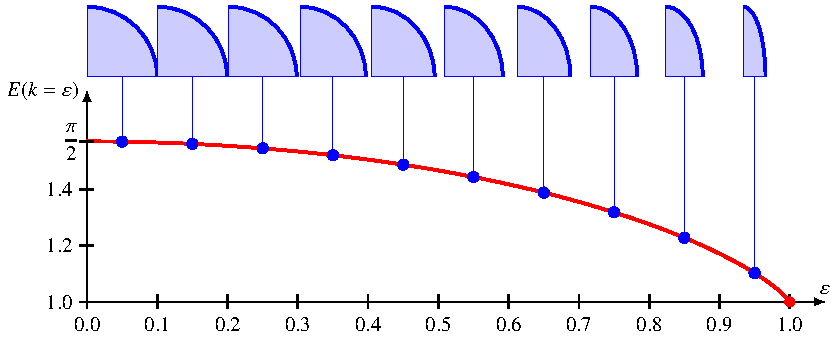
\includegraphics{chapters/110-elliptisch/images/ellipsenumfang.pdf}
\caption{Bogenlänge eines Viertels einer Ellipse mit Exzentrizität
$\varepsilon$.
Eine solche Ellipse hat Halbachsen $1$ und $\sqrt{1-\varepsilon^2}$,
ein entsprechender Ellipsenbogen ist für ausgewählte Werte in blau
eingezeichnet.
\label{buch:elliptisch:fig:ellipsenumfang}}
\end{figure}
Wir zeigen, wie sich die Berechnung des Umfangs $U$ einer Ellipse
mit Halbachsen $a$ und $b$, $a\le b$, auf ein volltändiges elliptisches
Integral zurückführen lässt.
Der Fall $a>b$ kann behandelt werden, indem die $x$- und $y$-Koordinaten
vertauscht werden.

Die Parametrisierung
\[
t\mapsto \begin{pmatrix}a\cos t\\ b\sin t\end{pmatrix}
\]
einer Ellipse führt auf das Integral
\begin{align}
U
&=
\int_0^{2\pi} \sqrt{a^2\sin^2t + b^2\cos^2 t}\,dt
\notag
\\
&=
4\int_0^{\frac{\pi}2}
\sqrt{a^2\sin^2t + b^2(1-\sin^2 t)}
\,dt
\notag
\\
&=
4b \int_0^{\frac{\pi}2} \sqrt{1-(b^2-a^2)/b^2\cdot \sin^2t}\,dt
\label{buch:elliptisch:eqn:umfangellipse}
\end{align}
für den Umfang der Ellipse.
Bei einem Kreis ist $a=b$ und der zweite Term unter der Wurzel fällt weg,
der Umfang wird $4b\frac{\pi}2=2\pi b$.
Die Differenz $e^2=b^2-a^2$ ist die {\em lineare Exzentrizität} der Ellipse,
\index{lineare Exzentrizität}%
der Quotient $e/b$ wird die {\em numerische Exzentrizität} der Ellipse
genannt.
Insbesondere ist $k = \varepsilon$.

Das Integral~\eqref{buch:elliptisch:eqn:umfangellipse} erhält jetzt die
Form
\[
U
=
4b\int_0^{\frac{\pi}2} \sqrt{1-k^2\sin^2t}\,dt
\]
und ist damit als elliptisches Integral zweiter Art erkannt.
Für den Umfang der Ellipse finden wir damit die Formel
\[
U
=
4b E(k)
=
4b E(\varepsilon).
\]
Das vollständige elliptische Integral zweiter Art $E(\varepsilon)$
liefert also genau den Umfang eines Viertels der Ellipse mit
numerischer Exzentrizität $\varepsilon$ und kleiner Halbachse $1$.
Für den extremen Wert $\varepsilon=0$ entsteht der Umfang einer Ellipse,
also $E(0)=\frac{\pi}2$.
Für $\varepsilon=1$ ist $a=0$, es entsteht eine Strecke mit Länge $E(1)=1$.

\begin{satz}
\label{buch:elliptisch:satz:hyperE}
Das vollständige elliptische Integral $E(k)$ ist
\[
E(k)
=
\int_0^{\frac{\pi}2} \sqrt{1-k^2\sin^2\vartheta}\,d\vartheta
=
\frac{\pi}2
\cdot
\mathstrut_2F_1\biggl(
\begin{matrix}-\frac12,\frac12\\1\end{matrix};
k^2
\biggr).
\]
\end{satz}

\begin{proof}[Beweis]
Die Identität kann wie im Satz~\ref{buch:elliptisch:satz:hyperK} mit
Hilfe einer Entwicklung der Wurzel mit der Binomialreihe gefunden
werden.
\end{proof}

Die Darstellung von $E(k)$ als hypergeometrische Reihe ermöglicht
jetzt zum Beispiel auch die Berechnung der Ableitung nach dem
Parameter $k$ mit der Ableitungsformel für die Funktion $\mathstrut_2F_1$.


%
% Berechnung mit dem arithmetisch-geometrischen Mittel
%
\subsection{Berechnung mit dem arithmetisch-geometrischen Mittel
\label{buch:elliptisch:subsection:agm}}
Die numerische Berechnung von elliptischer Integrale mit gewöhnlichen
numerischen Integrationsroutinen ist nicht sehr effizient.
Das in diesem Abschnitt vorgestellte arithmetisch-geometrische Mittel
\index{arithmetisch-geometrisches Mittel}%
liefert einen Algorithmus mit sehr viel besserer Konvergenz.
Die Methode lässt sich auch auf die unvollständigen elliptischen
Integrale von Abschnitt~\eqref{buch:elliptisch:subsection:unvollstintegral}
verallgemeinern.
Sie ist ein Speziallfall der sogenannten Landen-Transformation,
\index{Landen-Transformation}%
welche ausser für die elliptischen Integrale auch für die 
Jacobischen elliptischen Funktionen formuliert werden kann und
für letztere ebenfalls sehr schnelle numerische Algorithmen liefert
(siehe dazu auch die
Aufgaben~\ref{buch:elliptisch:aufgabe:2}--\ref{buch:elliptisch:aufgabe:4}).
Sie kann auch verwendet werden, um die Werte der Jacobischen elliptischen
Funktionen für komplexe Argument zu berechnen.
Eine weiter Anwendung ist die Berechnung einer grossen Zahl von 
Stellen der Kreiszahl $\pi$, siehe Aufgaben~\ref{buch:elliptisch:aufgabe:5}.

%
% Das arithmetisch-geometrische Mittel
%
\subsubsection{Das arithmetisch-geometrische Mittel}
Seien $a$ und $b$ zwei nichtnegative reelle Zahlen.
Aus $a$ und $b$ werden jetzt zwei Folgen konstruiert, deren Glieder
durch
\begin{align*}
a_0&=a &&\text{und}& a_{n+1} &= \frac{a_n+b_n}2 &&\text{arithmetisches Mittel}
\\
b_0&=b &&\text{und}& b_{n+1} &= \sqrt{a_nb_n}   &&\text{geometrisches Mittel}
\end{align*}
definiert sind.

\begin{satz}
\index{Satz!arithmetisch-geometrisches Mittel}%
Falls $a>b>0$ ist, nimmt die Folge $(a_k)_{k\ge 0}$ monoton ab und
$(b_k)_{k\ge 0}$ nimmt monoton zu.
Beide konvergieren quadratisch gegen einen gemeinsamen Grenzwert.
\end{satz}

\begin{definition}
Der gemeinsame Grenzwert von $a_n$ und $b_n$ heisst das
{\em arithmetisch-geometrische Mittel} und wird mit 
\[
M(a,b)
=
\lim_{n\to\infty} a_n
=
\lim_{n\to\infty} b_n
\]
bezeichnet.
\index{arithmetisch-geometrisches Mittel}%
\end{definition}

\begin{proof}[Beweis]
Zunächst ist zu zeigen, dass die Folgen monoton sind.
Dies folgt sofort aus der Definition der Folgen:
\begin{align*}
a_{n+1} &= \frac{a_n+b_n}{2} \ge \frac{a_n+a_n}{2} = a_n
\\
b_{n+1} &= \sqrt{a_nb_n} \ge \sqrt{b_nb_n} = b_n.
\end{align*}
Die Konvergenz folgt aus
\[
a_{n+1}-b_{n+1}
\le
a_{n+1}-b_n
=
\frac{a_n+b_n}{2}-b_n
=
\frac{a_n-b_n}2
\le
\frac{a-b}{2^{n+1}}.
\]
Dies zeigt jedoch nur, dass die Konvergenz mindestens ein
Bit in jeder Iteration ist.
Aus
\[
a_{n+1}^2 - b_{n+1}^2
=
\frac{(a_n+b_n)^2}{4} - a_nb_n
=
\frac{a_n^2 -2a_nb_n+b_n^2}{4}
=
\frac{(a_n-b_n)^2}{4}
\]
folgt
\[
a_{n+1}-b_{n+1}
=
\frac{(a_n-b_n)^2}{2(a_{n+1}+b_{n+1})}.
\]
Da der Nenner gegen $2M(a,b)$ konvergiert, wird der Fehler für in
jeder Iteration quadriert, die Zahl korrekter Stellen verdoppelt sich
in jeder Iteration, es liegt also quadratische Konvergenz vor.
\end{proof}

%
% Transformation des elliptischen Integrals
%
\subsubsection{Transformation des elliptischen Integrals}
In diesem Abschnitt soll das Integral
\[
I(a,b)
=
\int_0^{\frac{\pi}2}
\frac{dt}{\sqrt{a^2\cos^2 t + b^2\sin^2t}}
\]
berechnet werden.
Es ist klar, dass
\[
I(sa,sb)
=
\frac{1}{s} I(a,b).
\]

Gauss hat gefunden, dass die Substitution
\begin{equation}
\sin t
=
\frac{2a\sin t_1}{a+b+(a-b)\sin^2 t_1}
\label{buch:elliptisch:agm:subst}
\end{equation}
zu
\begin{equation}
\frac{dt}{\sqrt{a^2_{\phantom{1}}\cos^2 t + b^2_{\phantom{1}} \sin^2 t}}
=
\frac{dt_1}{\sqrt{a_1^2\cos^2 t_1 + b_1^2 \sin^2 t_1}}
\label{buch:elliptisch:agm:dtdt1}
\end{equation}
führt.
Um dies nachzuprüfen, muss man zunächst
\eqref{buch:elliptisch:agm:subst}
nach $t_1$ ableiten, was
\[
\frac{d}{dt_1}\sin t
=
\cos t
\frac{dt}{dt_1}
\qquad\Rightarrow\qquad
\biggl(
\frac{d}{dt_1}\sin t
\biggr)^2
=
(1-\sin^2t)\biggl(\frac{dt}{dt_1}\biggr)^2
\]
ergibt.
Die Ableitung von $t$ nach $t_1$ kann auch aus
\eqref{buch:elliptisch:agm:dtdt1}
ableiten, es ist
\[
\biggl(
\frac{dt}{dt_1}
\biggr)^2
=
\frac{a^2_{\phantom{1}} \cos^2 t + b^2_{\phantom{1}} \sin^2 t}{a_1^2 \cos^2 t_1 + b_1^2 \sin^2 t_1}.
\]
Man muss also nachprüfen, dass
\begin{equation}
\frac{1}{1-\sin^2 t}
\frac{d}{dt_1}\sin t
=
\frac{a^2 \cos^2 t + b^2 \sin^2 t}{a_1^2 \cos^2 t_1 + b_1^2 \sin^2 t_1}.
\label{buch:elliptisch:agm:deq}
\end{equation}
Dazu muss man zunächst $a_1=(a+b)/2$, $b_1=\!\sqrt{ab}$ setzen.
Ausserdem muss man $\cos^2 t$ durch $1-\sin^2t$ ersetzen und
$\sin t$ durch \eqref{buch:elliptisch:agm:subst}.
Auch $\cos^2 t_1$ muss man durch $1-\sin^2t_1$ ersetzt werden.
Dann kann man nach einer langwierigen Rechnung, die sich am leichtesten
mit einem Computer-Algebra-System ausführen lässt finden, dass
\eqref{buch:elliptisch:agm:deq}
tatsächlich korrekt ist.

\begin{satz}
\index{Satz!Gauss-Integrale}%
\label{buch:elliptisch:agm:integrale}
Für $a_1=(a+b)/2$ und $b_1=\sqrt{ab}$ gilt
\[
\int_0^{\frac{\pi}2}
\frac{dt}{a^2\cos^2 t + b^2 \sin^2 t}
=
\int_0^{\frac{\pi}2}
\frac{dt_1}{a_1^2\cos^2 t_1 + b_1^2 \sin^2 t_1}.
\]
\end{satz}

Der Satz~\ref{buch:elliptisch:agm:integrale} zeigt, dass die Ersetzung
von $a$ und $b$ durch $a_1$ und $b_1$ das Integral $I(a,b)$ nicht ändert.
Dies gilt natürlich für alle Glieder der Folge zur Bestimmung des
arithmetisch-geometrischen Mittels.

\begin{satz}
\index{Satz!Iab@$I(a,b)$ und arithmetisch geometrisches Mittel}%
Für $a\ge b>0$ gilt
\begin{equation}
I(a,b)
=
\int_0^{\frac{\pi}2}
\frac{dt}{a^2\cos^2 t + b^2\sin^2t}
=
\frac{\pi}{2M(a,b)}.
\end{equation}
\end{satz}

\begin{proof}[Beweis]
Zunächst folgt aus Satz~\ref{buch:elliptisch:agm:integrale}, dass
\[
I(a,b)
=
I(a_1,b_1)
=
\dots
=
I(a_n,b_n).
\]
Ausserdem ist $a_n\to M(a,b)$ und $b_n\to M(a,b)$,
damit wird 
\[
I(a,b)
=
\frac{1}{M(a,b)}
\int_0^{\frac{\pi}2}
\frac{dt}{\sqrt{\cos^2 t + \sin^2 t}}
=
\frac{\pi}{2M(a,b)}.
\qedhere
\]
\end{proof}

%
%  Berechnung des elliptischen Integrals
%
\subsubsection{Berechnung des elliptischen Integrals}
Das elliptische Integral erster Art hat eine Form, die dem Integral
$I(a,b)$ bereits sehr ähnlich ist.
Im die Verbindung herzustellen, berechnen wir
\begin{align*}
I(a,b)
&=
\int_0^{\frac{\pi}2}
\frac{dt}{\sqrt{a^2\cos^2 t + b^2 \sin^2 t}}
\\
&=
\frac{1}{a}
\int_0^{\frac{\pi}2}
\frac{dt}{\sqrt{1-\sin^2 t + \frac{b^2}{a^2} \sin^2 t}}
\\
&=
\frac{1}{a}
\int_0^{\frac{\pi}2}
\frac{dt}{\sqrt{1-(1-\frac{b^2}{a^2})\sin^2 t}}
=
K(k)
\qquad\text{mit}\qquad
k'=\frac{b^2}{a^2},\;
k=\sqrt{1-k^{\prime 2}}.
\end{align*}

\begin{satz}
\index{Satz!vollständige elliptische Integrale und arithmetisch-geometrisches Mittel}%
\label{buch:elliptisch:agm:satz:Ek}
Für $0<k\le 1$ ist
\[
K(k) = I(1,\sqrt{1-k^2}) = \frac{\pi}{2M(1,\sqrt{1-k^2})}.
\]
\end{satz}

%
% Numerisches Beispiel
%
\subsubsection{Numerisches Beispiel}
\begin{table}
\centering
\begin{tabular}{|>{$}c<{$}|>{$}c<{$}|>{$}c<{$}|>{$}c<{$}|}
\hline
n& a_n & b_n & \pi/2a_n \mathstrut\text{\vrule height12pt depth6pt width0pt}\\
\hline
\text{\vrule height12pt depth0pt width0pt}%
0 & 1.0000000000000000000 & 0.7071067811865475243 & 1.5707963267948965579 \\
1 & 0.8535533905932737621 & 0.8408964152537145430 & 1.\underline{8}403023690212201581 \\
2 & 0.8472249029234941526 & 0.8472012667468914603 & 1.\underline{8540}488143993356315 \\
3 & 0.8472130848351928064 & 0.8472130847527653666 & 1.\underline{854074677}2111781089 \\
4 & 0.8472130847939790865 & 0.8472130847939790865 & 1.\underline{854074677301371}8463 \\
\infty&                       &                       &          1.8540746773013719184%
\text{\vrule height12pt depth6pt width0pt}\\
\hline
\end{tabular}
\caption{Die Berechnung des arithmetisch-geometrischen Mittels für
$a=1$ und $b=\sqrt{2}/2$ zeigt die sehr rasche Konvergenz.
\label{buch:elliptisch:agm:numerisch}}
\end{table}
In diesem Abschnitt soll als Zahlenbeispiel $E(k)$ für $k=\sqrt{2}/2$
berechnet werden.
In diesem speziellen Fall ist $k'=k$.
Tabelle~\ref{buch:elliptisch:agm:numerisch} zeigt die sehr rasche
Konvergenz der Berechnung des arithmetisch-geometrischen Mittels
von $1$ und $\sqrt{2}/2$.
Mit Satz~\ref{buch:elliptisch:agm:satz:Ek} folgt jetzt
\[
K(\!\sqrt{2}/2)
=
\frac{\pi}{2M(1,\!\sqrt{2}/2)}
=
1.854074677301372.
\]
Die Berechnung hat nur 4 Mittelwerte, 4 Produkte, 4 Quadratwurzeln und
eine Division erfordert.

%
% Unvollständige elliptische Integrale
%
\subsection{Unvollständige elliptische Integrale
\label{buch:elliptisch:subsection:unvollstintegral}}
Die Funktionen $K(k)$ und $E(k)$ sind als bestimmte Integrale über ein
festes Intervall definiert.
Die {\em unvollständigen elliptischen Integrale} entstehen, indem die
\index{unvollständiges elliptisches Integral}%
obere Grenze des Integrals variabel wird:
\[
\begin{aligned}
\text{1.~Art:}&&
F(x,k)
&=
\int_0^x \frac{dt}{\sqrt{(1-t^2)(1-k^2t^2)}}
&&=
\int_0^\varphi \frac{d\vartheta}{\sqrt{1-k^2\sin^2\vartheta}}
\\
\text{2.~Art:}&&
E(x,k)
&=
\int_0^x \sqrt{\frac{1-k^2t^2}{1-t^2}}\,dt
&&=
\int_0^\varphi \sqrt{1-k^2\sin^2\vartheta}\,d\vartheta
\\
\text{3.~Art:}&&
\Pi(n,x,k)
&=
\int_0^x \frac{dt}{(1-nt^2)\sqrt{(1-t^2)(1-k^2t^2)}}
&&=
\int_0^\varphi
\frac{d\vartheta}{(1-n\sin^2\vartheta)\sqrt{1-k^2\sin^2\vartheta}},
\end{aligned}
\]
die erste Formel ist jeweils die Jacobi-Form, die zweite die Legrendre-Form
\index{Jacobi-Form}%
\index{Legendre-Form}%
mit dem Parameter $\varphi$, gegeben durch
$\sin \vartheta=x$.
Wie bei den vollständigen elliptischen Integralen ist auch hier in manchen
Referenzen die Parameterkonvention mit dem Parameter $m=k^2$ üblich.

Die vollständigen elliptischen Integrale sind die Werte der 
unvollständigen elliptischen Integrale mit $x=1$, also
\begin{align*}
K(k) &= F(1,k),
&
E(k) &= E(1,k),
&
\Pi(n,k) &=\Pi(n,x,k).
\end{align*}
Man beachte auch, dass $F(x,0) = E(x,0)$ gilt.

\begin{figure}
\centering
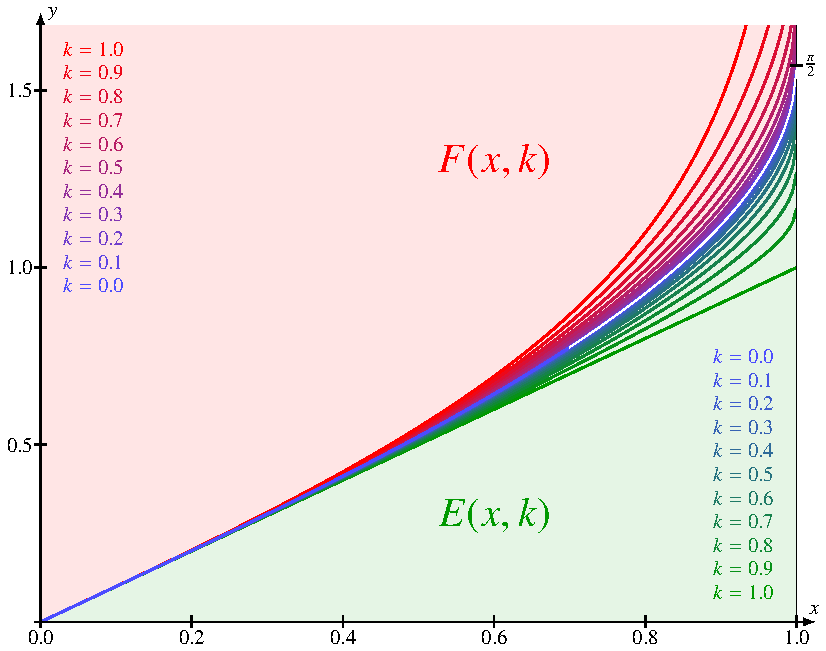
\includegraphics{chapters/110-elliptisch/images/unvollstaendig.pdf}
\caption{Unvollständige elliptische Integrale $F(x,k)$ und $E(x,k)$
für verschiedene Werte des Parameters $k$.
Für $k=0$ stimmen die Integrale erster und zweiter Art überein,
$F(x,0)=E(x,0)$.
\label{buch:elliptisch:fig:unvollstaendigeintegrale}}
\end{figure}
Wegen $k<1$ sind alle drei Integranden als reelle Funktionen nicht
mehr definiert, wenn $|x|>1$ ist.
Die Abbildung~\ref{buch:elliptisch:fig:unvollstaendigeintegrale}
zeigt Graphen der unvollständigen elliptischen Integrale für verschiedene
Werte des Parameters.

%
% Symmetrieeigenschaften
%
\subsubsection{Symmetrieeigenschaften}
Die Integranden aller drei unvollständigen elliptischen Integrale
sind gerade Funktionen der reellen Variablen $t$.
Die Funktionen $F(x,k)$, $E(x,k)$ und $\Pi(n,x,k)$ sind daher
ungeraden Funktionen von $x$.

%
% Elliptische Integrale als komplexe Funktionen
%
\subsubsection{Elliptische Integrale als komplexe Funktionen}
Die unvollständigen elliptischen Integrale $F(x,k)$, $F(x,k)$ und $\Pi(n,x,k)$
in Jacobi-Form lassen sich auch für komplexe Argumente interpretieren.
Dazu muss für die Berechnung des Integrals ein Pfad in der komplexen
Ebene gewählt werden, der die Singulariätten des Integranden vermeidet.

Die Faktoren, die in den Integranden der unvollständigen elliptischen
Integrale vorkommen, haben Nullstellen bei $\pm1$, $\pm1/k$ und
$\pm 1/\sqrt{n}$

% XXX Additionstheoreme \\
% XXX Parameterkonventionen \\

%
% Wertebereich
%
\subsubsection{Wertebereich}
\label{buch:elliptische:subsubsection:wertebereich}
Die unvollständigen elliptischen Integrale betrachtet als reelle Funktionen
haben nur positive relle Werte.
Zum Beispiel nimmt das unvollständige elliptische Integral erster Art
$F(k,x)$ nur Werte zwischen $0$ und $K(k)$ an.
Wenn komplexe Werte zulässig sind, kann man das Integral auch über die 
Singularitäten bei $\pm 1$ und $\pm 1/k$ hinweg ausführen, erhält
dabe aber möglicherweise komplexe Werte, weil die Radikanden in den
Integralen negativ werden.
Die Schwierigkeit dabei ist, dass die Quadratwurzel nicht eindeutig ist.
Welcher Wert der im Zusammenhang richtige ist, hängt davon ab, wie wir
dorthin kommen.

Die reelle Achse teilt den Definitionsbereich der unvollständigen
elliptischen Integrale in die obere und die untere Halbebene.
die Werte für reelle Argument beschreiben daher den Rand der Wertebereichs
für Argumente in der oberen bzw.~untere Halbebene.
Indem wir die Werte der elliptischen Integrale für reelle Argumente
berechnen, können wir daher den Rand des Wertebereichs ermitteln.

Im folgenden diskutieren wir nur das elliptische Integral erster Art,
die anderen können in der gleichen Art behandelt werden.
Für Argumentwerte $x$ im Interval $[0,1]$ ist $F(k,x)\in\mathbb{R}$.
An der Stelle $x=1$ wechselt der Faktor $(1-t^2)$ im Nenner das
Vorzeichen, der Integrand wird negativ.
Für Argumente zwischen $1$ und $1/k$ ist bleibt der Integrand negativ,
es muss also ein Wert der Quadratwurzel gewählt werden.
Beide Vorzeichen von
\begin{equation}
\frac{1}{\sqrt{(1-t^2)(1-k^2t^2)}}
=
\frac{\pm i}{\sqrt{(t^2-1)(1-k^2t^2)}}
\label{buch:elliptisch:eqn:imaginaerintegrand}
\end{equation}
sind möglich.
Doch welche Wahl ist die ``richtige''?

Dazu betrachten wir die Argument $z=x+i\varepsilon$ auf einer Geraden
parallel zur reellen Achse des Definitionsbereichs und in der oberen
Halbebene.
Da eine holomorphe Funktion die Orientierung erhält und weil das
Interval $[0,1]$ auf die reelle Achse abgebildet wird, müssen wir das
Vorzeichen der Wurzel so wählen, dass die Werte der Wurzel ebenfalls
in der oberen Halbebene liegen.
Die ``richtige'' Wahl der Wurzel von 
\[
1-z^2 = 1-x^2-2i\varepsilon x + \varepsilon^2
\]
erfüllt zwei Bedingungen.
\begin{enumerate}
\item
Für nicht zu grosse Werte von $x$ muss der Wert in der oberen
Halbebene liegen.
Für solche Werte von $x$ ist der Realteil $1-x^2+\varepsilon^2>0$ und
der Imaginärteil $-2\varepsilon x<0$.
Für die Wurzel muss man also das Argument von $1-z^2$ als Winkel zwischen
$3\pi2$ und $2\pi$ wählen und für die Wurzel durch zwei teilen.
\item
Der Realteil von $1-z^2$ wechsel das Vorzeichen, wenn
$x=\sqrt{1+\varepsilon^2}$, der Imaginärteil bleibt dabei negativ.
Das Argument ändert von einem Winkel nahe bei aber kleiner als $2\pi$
zu einem Winkel nahe bei aber grösser als $\pi$.
Als Wurzel muss daher jene verwendet werden, deren Argument in der
Nähe von $\frac{\pi}2$ liegt.
\end{enumerate}
Aus diesem Argument kann man ableiten, dass für die Berandung des
Bildes der oberen Halbebene zwischen $1$ und $1/k$ das positive
Zeichen in~\eqref{buch:elliptisch:eqn:imaginaerintegrand}
gewählt werden muss.

Die anderen Singularitäten auf der reellen Achse können analog
behandelt werden und es folgt, dass das Bild der oberen Halbebene
ein Rechteck in der oberen Halbebene ist
(Abbildung~\ref{buch:elliptisch:fig:rechteck}).
Die Ecken auf der reellen Achse liegen bei den reellen Koordinaten
\[
\pm F(1,k)
=
\pm\int_0^1\frac{dt}{\sqrt{(1-t^2)(1-k^2t^2)}}
=
\pm K(k).
\]
Für die Höhe muss das Integral
\begin{equation}
l({\textstyle\frac{1}{k}})=\int_1^{\frac1{k}}
\frac{dt}{\sqrt{(t^2-1)(1-k^2t^2)}}
\label{buch:elliptisch:eqn:hoeheintegral}
\end{equation}
ausgewertet werden.

%
% Komplementärmodul
%
\subsubsection{Komplementärmodul}
Im vorangegangen Abschnitt wurde gezeigt, dass der Wertebereicht des
unvollständigen elliptischen Integrals der ersten Art als komplexe
Funktion ein Rechteck ist.
Die obere Halbebene wird auf Rechteck der Breite $2K(k)$ abgebildet,
für die Höhe des Rechtecks muss das
Integral~\eqref{buch:elliptisch:eqn:hoeheintegral} ausgewertet werden.
Das Integral läuft von $t=1$ bis $t=1/k$, wir möchten daraus ein
elliptisches Integral machen, dessen Integrationsinterval bei $0$
beginnt.
Dazu verwenden wir die Variablentransformation
\[
t = \frac{1}{\sqrt{1-k'^2y^2}},
\]
die für $y=0$ den Wert $1$ ergibt, für $y=1$ aber $1/\sqrt{1-k'^2}$.
Damit das richtige Integrationsintervall entsteht, muss $k'$ so gewählt
werden, dass $1-k'^2=k^2$ ist.

\begin{definition}
Ist $0\le k\le 1$ der Modul eines elliptischen Integrals, dann heisst
$k' = \sqrt{1-k^2}$ der {\em Komplementärmodul} oder {\em Komplement
des Moduls}. Es ist $k^2+k'^2=1$.
\end{definition}

Mit der Ableitung
\[
\frac{dt}{dy}
=
\frac{k'^2 y}{(1-k'^2y^2)^{\frac32}}
\]
der Substitution
wird das Integral~\eqref{buch:elliptisch:eqn:hoeheintegral} mit der
oberen Grenze $x$ zu einem Integral mit oberer Grenze
\[
x^2 = \frac{1}{1-k'^2y_0^2}
\quad\Rightarrow\quad
y_0^2 = \frac{1}{k'^2}\biggl(1-\frac{1}{x^2}\biggr)
\quad\Rightarrow\quad
y_0=\frac{1}{k'}\sqrt{1-\frac{1}{x^2}}
\]
jetzt zu
\begin{align*}
l(x)
&=
\int_0^{y_0}
\frac{1}{\sqrt{\frac{1}{1-k'^2y^2}-1}}
\cdot
\frac{1}{\sqrt{1-\frac{k^2}{1-k'^2y^2}}}
\cdot
\frac{k'^2y}{\sqrt{1-k'^2y^2}}
\cdot
\frac{1}{1-k'^2y^2}
\,dy
\\
&=
\int_0^{y_0}
\frac{\sqrt{1-k'^2y^2}}{\sqrt{k'^2y^2}}
\cdot
\frac{1}{\sqrt{1-k^2 -k'^2y^2}}
\cdot
\frac{k'^2y}{1-k'^2y^2}
\,dy
\\
&=
\int_0^{y_0}
\sqrt{1-k'^2y^2}
\cdot
\frac{1}{k'\sqrt{1-y^2}}
\cdot
\frac{k'}{1-k'^2y^2}
\,dy
\\
&=
\int_0^{y_0} \frac{dy}{\sqrt{(1-y^2)(1-k'^2y^2)}}
=
F(y_0,k').
\end{align*}
Die gesuchte Höhe des Rechtecks ergibt sich für die obere Grenze $\frac1k$.
In diesem Fall ist
\[
y_0
=
\frac{1}{k'}\sqrt{1-k^2} = 1
\]
und das unvollständig elliptische Integral wird zum vollständigen
elliptischen Integral $K(k')$.
Die Höhe des Rechtecks des Wertebereichs der oberen Halbebene ist
als der Wert des vollständigen elliptischen Integrals erster Art
für den Komplementärmodul.
Das Bild der komplexen Ebene unter der Abbildung gegeben durch das
unvollständige elliptische Integral zweiter Art ist symmetrisch um
den Nullpunkt und hat Breite $2K(k)$ und Höhe $2K(k')$.

\begin{figure}
\centering
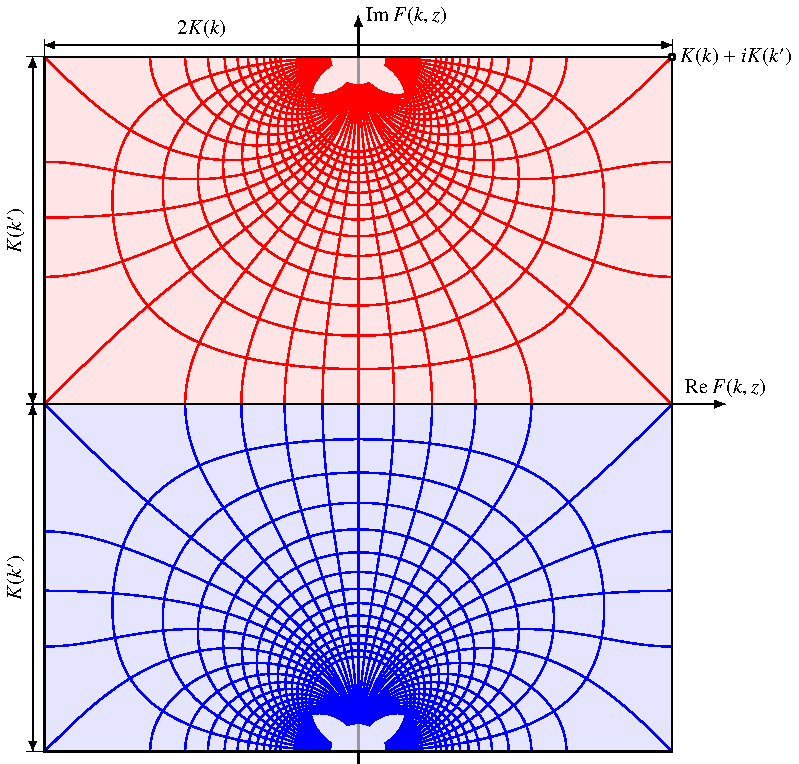
\includegraphics{chapters/110-elliptisch/images/rechteck.pdf}
\caption{Der Wertebereich der Funktion $F(k,z)$ ist ein Rechteck
der Breite $2K(k)$ und $2K(k')$.
Die obere Halbebene wird in das rote Rechteck abgebildet, die unter
in das blaue.
\label{buch:elliptisch:fig:rechteck}}
\end{figure}

%
% Reelle Argument > 1/k
%
\subsubsection{Reelle Argument $> 1/k$}
Für Argument $x> 1/k$ sind beide Faktoren im Integranden des 
unvollständigen elliptischen Integrals negativ, das Integral kann
daher wieder als gewöhnliches reelles Integral berechnet werden,
es sollte sich daher auch auf das unvollständige elliptische Integral
erster Art zurückführen lassen.

Da wir bereits wissen, dass 
\[
\lim_{x\to\infty} F(x,k) = iK(k'),
\]
können wir $F(x,k)$ auch als
\[
F(x,k)
=
iK(k')
-
\int_x^\infty \frac{dt}{\sqrt{(1-t^2)(1-k^2t^2)}}
\]
berechnen.
Dazu werden wir die Variablentransformation
\[
y=\frac{1}{kt}\quad\Leftrightarrow\quad t=\frac{1}{ky}
\qquad\text{mit}\qquad
\frac{dt}{dy} = -\frac{1}{ky^2}
\]
auf das Integral an und erhalten
\begin{align*}
\int_x^\infty \frac{dt}{\sqrt{(1-t^2)(1-k^2t^2)}}
&=
-\int_{\frac1{kx}}^0 \frac{dy}{ky^2\sqrt{(1-1/(ky)^2)(1-1/y^2)}}
\\
&=
\int_0^{\frac{1}{kx}} \frac{dy}{\sqrt{(k^2y^2-1)(y^2-1)}}
=
F\biggl(\frac{1}{kx},k\biggr).
\end{align*}
Dies ist das gesuchte unvollständige elliptische Integral erster Art.
Insbesondere halten wir noch die Formel
\[
F(x,k) = iK(k') - F\biggl(\frac1{kx},k\biggr)
\qquad\text{für $x>\frac1k$}
\]
für die Werte des elliptischen Integrals erster Art für grosse Argumentwerte
fest.

%
% AGM und Berechnung von F(x,k)
%
\subsubsection{Berechnung von $F(x,k)$ mit dem arithmetisch-geometrischen
Mittel\label{buch:elliptisch:subsubection:berechnung-fxk-agm}}
Wie das vollständige elliptische Integral $K(k)$ kann auch das  
unvollständige elliptische Integral
\begin{align*}
F(x,k)
&=
\int_0^x \frac{d\xi}{\sqrt{(1-\xi^2)(1-k^{\prime 2}\xi^2)}}
=
\int_0^{\varphi}
\frac{dt}{\sqrt{1-k^2 \sin^2 t}}
&&\text{mit $x=\sin\varphi$}
\\
&=
a
\int_0^{\varphi} \frac{dt}{a^2 \cos^2 t + b^2 \sin^2 t}
&&\text{mit $k=b/a$}
\end{align*}
mit dem arithmetisch-geometrischen Mittel berechnet werden.
Dazu muss die Substitution
\eqref{buch:elliptisch:agm:subst}
verwendet werden, um auch den Winkel $\varphi_1$ zu berechnen.
Zunächst wird \eqref{buch:elliptisch:agm:subst} nach $x_1=\sin t_1$ 
aufgelöst.
Durch Multiplikation mit dem Nenner erhält man mit der Abkürzung
$x=\sin t$ %und $x_1=\sin t_1$
die quadratische Gleichung
\[
(a-b)x x_1^2
-
2ax_1
+
(a+b)x 
=
0,
\]
mit der Lösung
\begin{equation}
x_1 
=
\frac{a-\sqrt{a^2-(a^2-b^2)x^2}}{(a-b)x}.
\label{buch:elliptisch:unvollstagm:xrek}
\end{equation}
Der Algorithmus zur Berechnung des arithmetisch-geometrischen Mittels
muss daher verallgemeinert werden zu
\begin{equation}
\left.
\begin{aligned}
a_{n+1} &= \frac{a_n+b_n}2,  &\qquad a_0 &= a
\\
b_{n+1} &= \sqrt{a_nb_n},    & b_0 &= b
\\
x_{n+1} &= \frac{a_n-\sqrt{a_n^2-(a_n^2-b_n^2)x_n^2}}{(a_n-b_n)x_n}, & x_0 &= x
\end{aligned}
\quad
\right\}
\label{buch:elliptisch:unvollstagm:rek}
\end{equation}
Die Folge $x_n$ konvergiert gegen einen Wert $x_{\infty} = \lim_{n\to\infty} x_n$.
Der Wert des unvollständigen elliptischen Integrals ist dann der Grenzwert
\[
F(x,k)
=
\lim_{n\to\infty}
\frac{\arcsin x_n}{M(a_n,b_n)}
=
\frac{\arcsin x_{\infty}}{M(1,\sqrt{1-k^2})}.
\]

In dieser Form ist die Berechnung allerdings nicht praktisch durchführbar.
Das Problem ist, dass die Differenz $a_n-b_n$, die in 
\eqref{buch:elliptisch:unvollstagm:rek}
im Nenner vorkommt, sehr schnell gegen Null geht.
Ausserdem ist die Quadratwurzel im Zähler fast gleich gross wie
$a_n$, was zu Auslöschung und damit ungenauen Resultaten führt.
\label{buch:elliptisch:agm:ellintegral-stabilitaet}

Eine Möglichkeit, das Problem zu entschärfen, ist, die Rekursionsformel
nach $\varepsilon = a-b$ zu entwickeln.
Mit $a+b=2a+\varepsilon$ kann man $b$ aus der Formel elimineren und erhält
mit Hilfe der binomischen Reihe
\begin{align*}
x_1
&=
\frac{a}{x\varepsilon}
\left(1-\sqrt{1-\varepsilon(2a-\varepsilon)x^2/a^2}\right)
\\
&=
\frac{a}{x\varepsilon}
\biggl(
1-\sum_{k=0}^\infty
(-1)^k
\frac{(\frac12)_k}{k!} \varepsilon^k(2a-\varepsilon)^k\frac{x^{2k}}{a^{2k}}
\biggr)
\\
&=
\sum_{k=1}^\infty
(-1)^{k-1} 
\frac{(\frac12)_k}{k!} \varepsilon^{k-1}(2a-\varepsilon)^k\frac{x^{2k-1}}{a^{2k-1}}
\\
&=
\frac{\frac12}{1!}(2a-\varepsilon)\frac{x}{a}
-
\frac{\frac12\cdot(\frac12-1)}{2!}\varepsilon(2a-\varepsilon)^2\frac{x^3}{a^3}
+
\frac{\frac12\cdot(\frac12-1)(\frac12-2)}{3!}\varepsilon^2(2a-\varepsilon)^3\frac{x^5}{a^5}
-
\dots
\\
&=
x\biggl(1-\frac{\varepsilon}{2a}\biggr)
\biggl(
1
-
\frac{\frac12-1}{2!}\varepsilon(2a-\varepsilon)\frac{x^2}{a^2}
+
\frac{(\frac12-1)(\frac12-2)}{3!}\varepsilon^2(2a-\varepsilon)^2\frac{x^4}{a^4}
-
\dots
\biggr)
\\
&=
x\biggl(1-\frac{\varepsilon}{2a}\biggr)
\cdot
\mathstrut_2F_1\biggl(
\begin{matrix}-\frac12,1\\2\end{matrix};-\varepsilon(2a-\varepsilon)\frac{x^2}{a^2}
\biggr).
\end{align*}
Diese Form ist wesentlich besser, aber leider kann es bei der numerischen
Rechnung passieren, dass $\varepsilon < 0$ wird.

%\subsection{Potenzreihe}
%XXX Potenzreihen \\
%XXX Als hypergeometrische Funktionen \url{https://www.youtube.com/watch?v=j0t1yWrvKmE} \\
%XXX Berechnung mit der Landen-Transformation https://en.wikipedia.org/wiki/Landen%27s_transformation


%
% jacobi.tex
%
% (c) 2021 Prof Dr Andreas Müller, OST Ostschweizer Fachhochschule
%
\section{Jacobische elliptische Funktionen
\label{buch:elliptisch:section:jacobi}}
\rhead{Jacobische elliptische Funktionen}
Die elliptischen Integrale von
Abschnitt~\ref{buch:elliptisch:section:integral}
können dazu verwendet werden, die Länge eines Ellipsenbogens aus
den Koordinaten der Endpunkte zu berechnen.
Die trigonometrischen Funktionen drücken dagegen umgekehrt die
Koordinaten eines Punktes auf einem Kreis aus der Länge des
Kreisbogens aus.
Das elliptische Integral, welches die Bogenlänge auf einer Ellipse zwischen
den Punkten $(1,0)$ und $(x,y)$ entsprecht also eher der Funktion
$\arcsin y=\sin^{-1}y$.
Möchte man Funktionen konstruieren, die die Eigenschaften der 
trigonometrischen Funktionen auf die Geometrie von Ellipsen erweitern,
dann muss man die Umkehrfunktionen der elliptischen Integrale dafür ins
Auge fassen.

%
% elltrigo.tex
%
% (c) 2022 Prof Dr Andreas Müller, OST Ostschweizer Fachhochschule
%

%
% elliptische Funktionen als Trigonometrie
%
\subsection{Elliptische Funktionen als Trigonometrie}
\begin{figure}
\centering
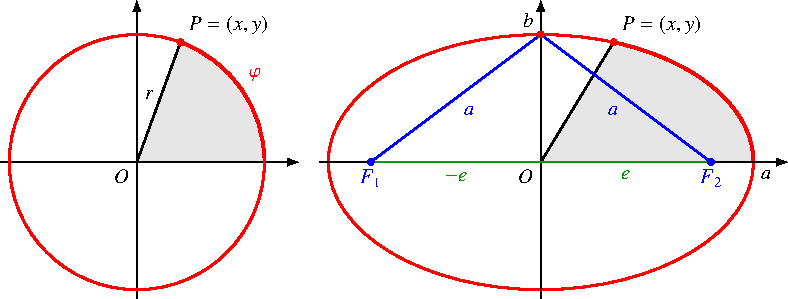
\includegraphics{chapters/110-elliptisch/images/ellipse.pdf}
\caption{Kreis und Ellipse zum Vergleich und zur Herleitung der 
elliptischen Funktionen von Jacobi als ``trigonometrische'' Funktionen
auf einer Ellipse.
\label{buch:elliptisch:fig:ellipse}}
\end{figure}
% based on Willliam Schwalm, Elliptic functions and elliptic integrals
% https://youtu.be/DCXItCajCyo
Die Ellipse wurde in Abschnitt~\ref{buch:geometrie:subsection:kegelschnitte}
als Kegelschnitt erkannt und auf verschiedene Arten parametrisiert.
In diesem Abschnitt soll gezeigt werden, wie man die Parametrisierung
eines Kreises mit trigonometrischen Funktionen verallgemeinern kann
auf eine Parametrisierung einer Ellipse mit den drei
Funktionen $\operatorname{sn}(u,k)$,
$\operatorname{cn}(u,k)$ und $\operatorname{dn}(u,k)$,
die ähnliche Eigenschaften haben wie die trigonometrischen Funktionen.

Die nachstehende Darstellung ist stark inspiriert von William Schwalms 
sehr zielorientierten Einführung
\cite{buch:schwalm}, welche auch als Youtube-Videovorlesung
\cite{buch:schwalm-youtube} zur Verfügung steht.

%
% Geometrie einer Ellipse
%
\subsubsection{Geometrie einer Ellipse}
Eine {\em Ellipse} ist die Menge der Punkte der Ebene, für die die Summe
\index{Ellipse}%
der Entfernungen von zwei festen Punkten $F_1$ und $F_2$,
den {\em Brennpunkten}, konstant ist.
\index{Brennpunkt}%
In Abbildung~\ref{buch:elliptisch:fig:ellipse} eine Ellipse
mit Brennpunkten in $F_1=(-e,0)$ und $F_2=(e,0)$ dargestellt,
die durch die Punkte $(\pm a,0)$ und $(0,\pm b)$ auf den Achsen geht.
Der Punkt $(a,0)$ hat die Entfernungen $a+e$ und $a-e$ von den beiden
Brennpunkten, also die Entfernungssumme $a+e+a-e=2a$.
Jeder andere Punkt auf der Ellipse muss ebenfalls diese Entfernungssumme
haben, insbesondere auch der Punkt $(0,b)$.
Seine Entfernung zu jedem Brennpunkt muss aus Symmetriegründen gleich gross,
also $a$ sein.
Aus dem Satz von Pythagoras liest man daher ab, dass
\[
b^2+e^2=a^2
\qquad\Rightarrow\qquad
e^2 = a^2-b^2
\]
sein muss.
Die Strecke $e$ heisst auch {\em (lineare) Exzentrizität} der Ellipse.
Das Verhältnis $\varepsilon= e/a$  heisst die {\em numerische Exzentrizität}
der Ellipse.

%
% Die Ellipsengleichung
%
\subsubsection{Ellipsengleichung}
Der Punkt $P=(x,y)$ auf der Ellipse hat die Entfernungen
\begin{equation}
\begin{aligned}
\overline{PF_1}^2
&=
y^2 + (x+e)^2
\\
\overline{PF_2}^2
&=
y^2 + (x-e)^2
\end{aligned}
\label{buch:elliptisch:eqn:wurzelausdruecke}
\end{equation}
von den Brennpunkten, für die 
\begin{equation}
\overline{PF_1}+\overline{PF_2}
=
2a
\label{buch:elliptisch:eqn:pf1pf2a}
\end{equation}
gelten muss.
Man kann nachrechnen, dass ein Punkt $P$, der die Gleichung
\[
\frac{x^2}{a^2} + \frac{y^2}{b^2}=1
\]
erfüllt, auch die Eigenschaft~\eqref{buch:elliptisch:eqn:pf1pf2a}
erfüllt.
Zur Vereinfachung setzen wir $l_1=\overline{PF_1}$ und $l_2=\overline{PF_2}$.
$l_1$ und $l_2$ sind Wurzeln aus der rechten Seite von
\eqref{buch:elliptisch:eqn:wurzelausdruecke}.
Das Quadrat von $l_1+l_2$ ist
\[
l_1^2 + 2l_1l_2 + l_2^2 = 4a^2.
\]
Um die Wurzeln ganz zu eliminieren, bringt man das Produkt $l_1l_2$ alleine
auf die rechte Seite und quadriert.
Man muss also verifizieren, dass
\[
(l_1^2 + l_2^2 -4a^2)^2 = 4l_1^2l_2^2.
\]
In den entstehenden Ausdrücken muss man ausserdem $e=\sqrt{a^2-b^2}$ und
\[
y=b\sqrt{1-\frac{x^2}{a^2}}
\]
substituieren.
Diese Rechnung führt man am einfachsten mit Hilfe eines
Computeralgebraprogramms durch, welches obige Behauptung bestätigt.

%
% Normierung
%
\subsubsection{Normierung}
Die trigonometrischen Funktionen sind definiert als Verhältnisse 
von Seiten rechtwinkliger Dreiecke.
Dadurch, dass man den die Hypothenuse auf Länge $1$ normiert, 
kann man die Sinus- und Kosinus-Funktion als Koordinaten eines
Punktes auf dem Einheitskreis interpretieren.

Für die Koordinaten eines Punktes auf der Ellipse ist dies nicht so einfach,
weil es nicht nur eine Ellipse gibt, sondern für jede numerische Exzentrizität
mindestens eine mit Halbachse $1$.
Wir wählen die Ellipsen so, dass $a$ die grosse Halbachse ist, also $a>b$.
Als Normierungsbedingung verwenden wir, dass $b=1$ sein soll, wie in
Abbildung~\ref{buch:elliptisch:fig:jacobidef}.
Dann ist $a=1/\varepsilon>1$.
In dieser Normierung haben Punkte $(x,y)$ auf der Ellipse $y$-Koordinaten
zwischen $-1$ und $1$ und $x$-Koordinaten zwischen $-a$ und $a$.

Im Zusammenhang mit elliptischen Funktionen wird die numerische Exzentrizität
$\varepsilon$ auch mit
\[
k
=
\varepsilon
=
\frac{e}{a}
=
\frac{\sqrt{a^2-b^2}}{a}
=
\frac{\sqrt{a^2-1}}{a},
\]
die Zahl $k$ heisst auch der {\em Modulus}.
Man kann $a$ auch durch $k$ ausdrücken, durch Quadrieren und Umstellen
findet man
\[
k^2a^2 = a^2-1
\quad\Rightarrow\quad
1=a^2(k^2-1)
\quad\Rightarrow\quad
a=\frac{1}{\sqrt{k^2-1}}.
\]

Die Gleichung der ``Einheitsellipse'' zu diesem Modulus ist
\[
\frac{x^2}{a^2}+y^2=1
\qquad\text{oder}\qquad
x^2(k^2-1) + y^2 = 1.
\]

%
% Definition der elliptischen Funktionen
%
\begin{figure}
\centering
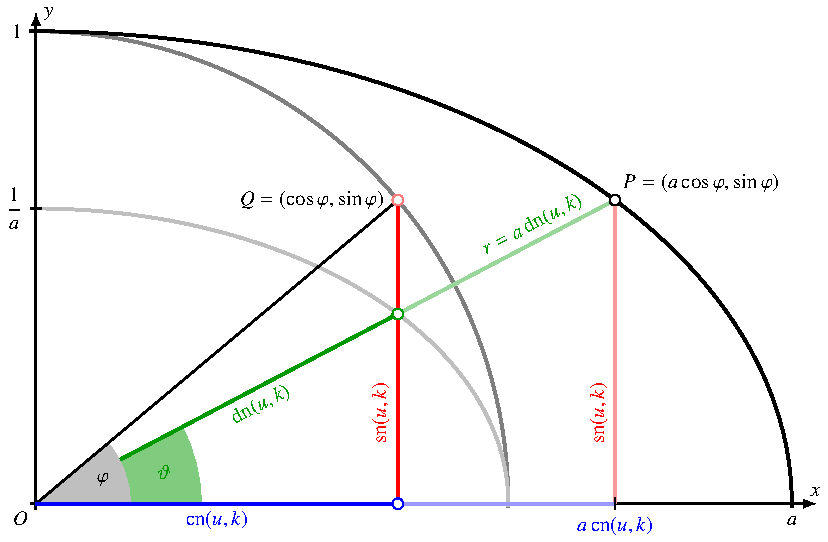
\includegraphics{chapters/110-elliptisch/images/jacobidef.pdf}
\caption{Definition der elliptischen Funktionen als Trigonometrie
an einer Ellipse mit Halbachsen $a$ und $1$.
\label{buch:elliptisch:fig:jacobidef}}
\end{figure}
\subsubsection{Definition der Jacobischen elliptischen Funktionen}
Die elliptischen Funktionen für einen Punkt $P$ auf der Ellipse mit Modulus $k$
können jetzt als Verhältnisse der Koordinaten des Punktes definieren.
Es stellt sich aber die Frage, was man als Argument verwenden soll.
Es soll so etwas wie den Winkel $\varphi$ zwischen der $x$-Achse und dem
Radiusvektor zum Punkt $P$
darstellen, aber wir haben hier noch eine Wahlfreiheit, die wir später
ausnützen möchten.
Im Moment müssen wir die Frage noch nicht beantworten und nennen das
noch unbestimmte Argument $u$.
Wir kümmern uns später um die Frage, wie $u$ von $\varphi$ abhängt.

Die Funktionen, die wir definieren wollen, hängen ausserdem auch 
vom Modulus ab.
Falls der verwendete Modulus aus dem Zusammenhang klar ist, lassen
wir das $k$-Argument weg.

Die Punkte auf dem Einheitskreis haben alle den gleichen Abstand vom
Nullpunkt, dies ist gleichzeitig die definierende Gleichung $r^2=x^2+y^2=1$
des Kreises.
Die Punkte auf der Ellipse erfüllen die Gleichung $x^2/a^2+y^2=1$,
die Entfernung der Punkte $r=\sqrt{x^2+y^2}$ vom Nullpunkt variert aber.

In Analogie zu den trigonometrischen Funktionen setzen wir jetzt für 
die Funktionen
\[
\begin{aligned}
&\text{sinus amplitudinis:}&
{\color{red}\operatorname{sn}(u,k)}&= y \\
&\text{cosinus amplitudinis:}&
{\color{blue}\operatorname{cn}(u,k)}&= \frac{x}{a} \\
&\text{delta amplitudinis:}&
{\color{darkgreen}\operatorname{dn}(u,k)}&=\frac{r}{a},
\end{aligned}
\]
die auch in Abbildung~\ref{buch:elliptisch:fig:jacobidef}
dargestellt sind.
Aus der Gleichung der Ellipse folgt sofort, dass
\[
\operatorname{sn}(u,k)^2 + \operatorname{cn}(u,k)^2 = 1
\]
ist.
Der Satz von Pythagoras kann verwendet werden, um die Entfernung zu
berechnen, also gilt
\begin{equation}
r^2
=
a^2 \operatorname{dn}(u,k)^2
=
x^2 + y^2
=
a^2\operatorname{cn}(u,k)^2 + \operatorname{sn}(u,k)^2
\quad
\Rightarrow
\quad
a^2 \operatorname{dn}(u,k)^2
=
a^2\operatorname{cn}(u,k)^2 + \operatorname{sn}(u,k)^2.
\label{buch:elliptisch:eqn:sncndnrelation}
\end{equation}
Ersetzt man
$
a^2\operatorname{cn}(u,k)^2
=
a^2-a^2\operatorname{sn}(u,k)^2
$, ergibt sich
\[
a^2 \operatorname{dn}(u,k)^2
=
a^2-a^2\operatorname{sn}(u,k)^2
+
\operatorname{sn}(u,k)^2
\quad
\Rightarrow
\quad
\operatorname{dn}(u,k)^2
+
\frac{a^2-1}{a^2}\operatorname{sn}(u,k)^2
=
1,
\]
woraus sich die Identität
\[
\operatorname{dn}(u,k)^2 + k^2 \operatorname{sn}(u,k)^2 = 1
\]
ergibt.
Ebenso kann man aus~\eqref{buch:elliptisch:eqn:sncndnrelation}
die Funktion $\operatorname{cn}(u,k)$ eliminieren, was auf
\[
a^2\operatorname{dn}(u,k)^2
=
a^2\operatorname{cn}(u,k)^2
+1-\operatorname{cn}(u,k)^2
=
(a^2-1)\operatorname{cn}(u,k)^2
+1.
\]
Nach Division durch $a^2$ ergibt sich
\begin{align*}
\operatorname{dn}(u,k)^2
-
k^2\operatorname{cn}(u,k)^2
&=
\frac{1}{a^2}
=
\frac{a^2-a^2+1}{a^2}
=
1-k^2 =: k^{\prime 2}.
\end{align*}
Wir stellen die hiermit gefundenen Relationen zwischen den grundlegenden
Jacobischen elliptischen Funktionen für später zusammen in den Formeln
\begin{equation}
\begin{aligned}
\operatorname{sn}^2(u,k)
+
\operatorname{cn}^2(u,k)
&=
1
\\
\operatorname{dn}^2(u,k) + k^2\operatorname{sn}^2(u,k)
&=
1
\\
\operatorname{dn}^2(u,k)  -k^2\operatorname{cn}^2(u,k)
&=
k^{\prime 2}.
\end{aligned}
\label{buch:elliptisch:eqn:jacobi-relationen}
\end{equation}
zusammen.
So wie es möglich ist, $\sin\alpha$ durch $\cos\alpha$ auszudrücken,
ist es mit
\eqref{buch:elliptisch:eqn:jacobi-relationen}
jetzt auch möglich jede grundlegende elliptische Funktion durch
jede anderen auszudrücken.
Die Resultate sind in der Tabelle~\ref{buch:elliptisch:fig:jacobi-relationen}
zusammengestellt.

\begin{table}
\centering
\renewcommand{\arraystretch}{2.1}
\begin{tabular}{|>{$\displaystyle}c<{$}|>{$\displaystyle}c<{$}>{$\displaystyle}c<{$}>{$\displaystyle}c<{$}|}
\hline
&\operatorname{sn}(u,k)
&\operatorname{cn}(u,k)
&\operatorname{dn}(u,k)\\
\hline
\operatorname{sn}(u,k)
&\operatorname{sn}(u,k)
&\sqrt{1-\operatorname{cn}^2(u,k)}
&\frac1k\sqrt{1-\operatorname{dn}^2(u,k)}
\\
\operatorname{cn}(u,k)
&\sqrt{1-\operatorname{sn}^2(u,k)}
&\operatorname{cn}(u,k)
&\frac{1}{k}\sqrt{\operatorname{dn}^2(u,k)-k^{\prime2}}
\\
\operatorname{dn}(u,k)
&\sqrt{1-k^2\operatorname{sn}^2(u,k)}
&\sqrt{k^{\prime2}+k^2\operatorname{cn}^2(u,k)}
&\operatorname{dn}(u,k)
\\
\hline
\end{tabular}
\caption{Jede der Jacobischen elliptischen Funktionen lässt sich
unter Verwendung der Relationen~\eqref{buch:elliptisch:eqn:jacobi-relationen}
durch jede andere ausdrücken.
\label{buch:elliptisch:fig:jacobi-relationen}}
\end{table}

%
% Ableitungen der Jacobi-ellpitischen Funktionen
% 
\subsubsection{Ableitung}
Die trigonometrischen Funktionen sind deshalb so besonders nützlich 
für die Lösung von Schwingungsdifferentialgleichungen, weil sie die
Beziehungen
\[
\frac{d}{d\varphi}  \cos\varphi = -\sin\varphi
\qquad\text{und}\qquad
\frac{d}{d\varphi}  \sin\varphi = \cos\varphi
\]
erfüllen.
So einfach können die Beziehungen natürlich nicht sein, sonst würde sich
durch Integration ja wieder nur die trigonometrischen Funktionen ergeben.
Durch geschickte Wahl des Arguments $u$ kann man aber erreichen, dass
sie ähnlich nützliche Beziehungen zwischen den Ableitungen ergeben.

Gesucht ist jetzt also eine Wahl für das Argument $u$ zum Beispiel in
Abhängigkeit von $\varphi$, dass sich einfache und nützliche
Ableitungsformeln ergeben.
Wir setzen daher $u(\varphi)$ voraus und beachten, dass $x$ und $y$
ebenfalls von $\varphi$ abhängen, es ist
$y=\sin\varphi$ und $x=a\cos\varphi$.
Die Ableitungen von $x$ und $y$ nach $\varphi$ sind
\begin{align*}
\frac{dy}{d\varphi}
&=
\cos\varphi
=
\frac{1}{a} x
=
\operatorname{cn}(u,k)
\\
\frac{dx}{d\varphi}
&=
-a\sin\varphi
=
-a y
=
-a\operatorname{sn}(u,k).
\end{align*}
Daraus kann man jetzt die folgenden Ausdrücke für die Ableitungen der
elliptischen Funktionen nach $\varphi$ ableiten:
\begin{align*}
\frac{d}{d\varphi} \operatorname{sn}(u,z)
&=
\frac{d}{d\varphi} y(\varphi)
=
\cos\varphi
=
\frac{x}{a}
=
\operatorname{cn}(u,k)
&&\Rightarrow&
\frac{d}{du}
\operatorname{sn}(u,k)
&=
\operatorname{cn}(u,k) \frac{d\varphi}{du}
\\
\frac{d}{d\varphi} \operatorname{cn}(u,z)
&=
\frac{d}{d\varphi} \frac{x(\varphi)}{a}
=
-\sin\varphi
=
-\operatorname{sn}(u,k)
&&\Rightarrow&
\frac{d}{du}\operatorname{cn}(u,k)
&=
-\operatorname{sn}(u,k) \frac{d\varphi}{du}
\\
\frac{d}{d\varphi} \operatorname{dn}(u,z)
&=
\frac{1}{a}\frac{dr}{d\varphi}
=
\frac{1}{a}\frac{d\sqrt{x^2+y^2}}{d\varphi}
%\\
%&
\rlap{$\displaystyle\mathstrut
=
\frac{x}{ar} \frac{dx}{d\varphi}
+
\frac{y}{ar} \frac{dy}{d\varphi}
%\\
%&
=
\frac{x}{ar} (-a\operatorname{sn}(u,k))
+
\frac{y}{ar} \operatorname{cn}(u,k)
$}
\\
&
\rlap{$\displaystyle\mathstrut
=
\frac{x}{ar}(-ay)
+
\frac{y}{ar} \frac{x}{a}
%\rlap{$\displaystyle
=
\frac{xy(-1+\frac{1}{a^2})}{r} 
%$}
%\\
%&
=
-\frac{xy(a^2-1)}{a^2r} 
$}
\\
&=
-\frac{a^2-1}{ar}
\operatorname{cn}(u,k) \operatorname{sn}(u,k)
%\\
%&
\rlap{$\displaystyle\mathstrut
=
-k^2
\frac{a}{r}
\operatorname{cn}(u,k) \operatorname{sn}(u,k)
$}
\\
&=
-k^2\frac{\operatorname{cn}(u,k)\operatorname{sn}(u,k)}{\operatorname{dn}(u,k)}
&&\Rightarrow&
\frac{d}{du} \operatorname{dn}(u,k)
&=
-k^2\frac{\operatorname{cn}(u,k)
\operatorname{sn}(u,k)}{\operatorname{dn}(u,k)}
\frac{d\varphi}{du}.
\end{align*}
Die einfachsten Beziehungen ergeben sich offenbar, wenn man $u$ so
wählt, dass
\[
\frac{d\varphi}{du}
=
\operatorname{dn}(u,k)
=
\frac{r}{a}.
\]
Damit haben wir die im folgenden Satz zusammengefassten
grundlegenden Ableitungsregeln der Jacobischen elliptischen Funktionen
gefunden.

\begin{satz}
\index{Satz!Ableitungen der Jacobischen elliptischen Funktionen}%
\label{buch:elliptisch:satz:ableitungen}
Die Jacobischen elliptischen Funktionen haben die Ableitungen
\begin{equation}
\begin{aligned}
\frac{d}{du}\operatorname{sn}(u,k)
&=
\phantom{-}\operatorname{cn}(u,k)\operatorname{dn}(u,k)
\\
\frac{d}{du}\operatorname{cn}(u,k)
&=
-\operatorname{sn}(u,k)\operatorname{dn}(u,k)
\\
\frac{d}{du}\operatorname{dn}(u,k)
&=
-k^2\operatorname{sn}(u,k)\operatorname{cn}(u,k).
\end{aligned}
\label{buch:elliptisch:eqn:ableitungsregeln}
\end{equation}
\end{satz}

%
% Der Grenzfall $k=1$
%
\subsubsection{Der Grenzwert $k\to1$}
\begin{figure}
\centering
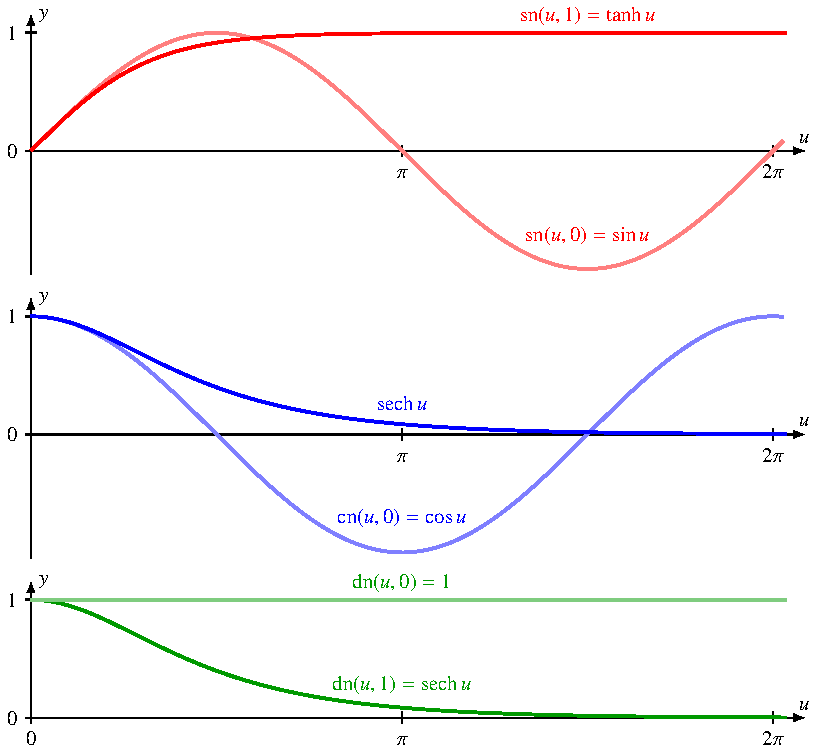
\includegraphics{chapters/110-elliptisch/images/sncnlimit.pdf}
\caption{Grenzfälle der Jacobischen elliptischen Funktionen 
für die Werte $0$ und $1$ des Parameters $k$.
\label{buch:elliptisch:fig:sncnlimit}}
\end{figure}
Für $k=1$ ist $k^{\prime2}=1-k^2=$ und es folgt aus den
Relationen~\eqref{buch:elliptisch:eqn:jacobi-relationen}
\[
\operatorname{cn}^2(u,k)
-
k^2
\operatorname{dn}^2(u,k)
=
k^{\prime2}
=
0
\qquad\Rightarrow\qquad
\operatorname{cn}^2(u,1)
=
\operatorname{dn}^2(u,1),
\]
die beiden Funktionen
$\operatorname{cn}(u,k)$
und
$\operatorname{dn}(u,k)$
fallen also zusammen.
Die Ableitungsregeln werden dadurch vereinfacht:
\begin{align*}
\operatorname{sn}'(u,1)
&=
\operatorname{cn}(u,1)
\operatorname{dn}(u,1)
=
\operatorname{cn}^2(u,1)
=
1-\operatorname{sn}^2(u,1)
&&\Rightarrow& y'&=1-y^2
\\
\operatorname{cn}'(u,1)
&=
-
\operatorname{sn}(u,1)
\operatorname{dn}(u,1)
=
-
\operatorname{sn}(u,1)\operatorname{cn}(u,1)
&&\Rightarrow&
\frac{z'}{z}&=(\log z)' = -y.
\end{align*}
Die erste Differentialgleichung für $y$ lässt sich separieren, man findet
die Lösung
\[
\frac{y'}{1-y^2}
=
1
\quad\Rightarrow\quad
\int \frac{dy}{1-y^2} = \int \,du
\quad\Rightarrow\quad
\operatorname{artanh}(y) = u
\quad\Rightarrow\quad
\operatorname{sn}(u,1)=\tanh u.
\]
Damit kann man jetzt auch $z$ berechnen:
\begin{align*}
(\log \operatorname{cn}(u,1))'
&=
\tanh u
&&\Rightarrow&
\log\operatorname{cn}(u,1)
&=
-\int\tanh u\,du
=
-\log\cosh u
\\
&
&&\Rightarrow&
\operatorname{cn}(u,1)
&=
\frac{1}{\cosh u}
=
\operatorname{sech}u.
\end{align*}
Die Grenzfunktionen sind in Abbildung~\ref{buch:elliptisch:fig:sncnlimit}
dargestellt.

%
% Das Argument u
%
\subsubsection{Das Argument $u$}
Die Gleichung 
\begin{equation}
\frac{d\varphi}{du}
=
\operatorname{dn}(u,k)
\label{buch:elliptisch:eqn:uableitung}
\end{equation}
ermöglicht, $\varphi$ in Abhängigkeit von $u$ zu berechnen, ohne jedoch
die geometrische Bedeutung zu klären.
Das beginnt bereits damit, dass der Winkel $\varphi$ nicht nicht der
Polarwinkel des Punktes $P$ in Abbildung~\ref{buch:elliptisch:fig:jacobidef}
ist, diesen nennen wir $\vartheta$.
Der Zusammenhang zwischen $\varphi$ und $\vartheta$ ist
\begin{equation}
\frac1{a}\tan\varphi = \tan\vartheta.
\label{buch:elliptisch:eqn:phitheta}
\end{equation}

Um die geometrische Bedeutung besser zu verstehen, nehmen wir jetzt an,
dass die Ellipse mit einem Parameter $t$ parametrisiert ist, dass also
$\varphi(t)$, $\vartheta(t)$ und $u(t)$ Funktionen von $t$ sind.
Die Ableitung von~\eqref{buch:elliptisch:eqn:phitheta} ist
\[
\frac1{a}\cdot \frac{1}{\cos^2\varphi}\cdot \dot{\varphi}
=
\frac{1}{\cos^2\vartheta}\cdot \dot{\vartheta}.
\]
Daraus kann die Ableitung von $\vartheta$ nach $\varphi$ bestimmt
werden, sie ist
\[
\frac{d\vartheta}{d\varphi}
=
\frac{\dot{\vartheta}}{\dot{\varphi}}
=
\frac{1}{a}
\cdot
\frac{\cos^2\vartheta}{\cos^2\varphi}
=
\frac{1}{a}
\cdot
\frac{(x/r)^2}{(x/a)^2}
=
\frac{1}{a}\cdot
\frac{a^2}{r^2}
=
\frac{1}{a}\cdot\frac{1}{\operatorname{dn}^2(u,k)}.
\]
Damit kann man jetzt mit Hilfe von~\eqref{buch:elliptisch:eqn:uableitung} 
Die Ableitung von $\vartheta$ nach $u$ ermitteln, sie ist
\[
\frac{d\vartheta}{du}
=
\frac{d\vartheta}{d\varphi}
\cdot
\frac{d\varphi}{du}
=
\frac{1}{a}\cdot\frac{1}{\operatorname{dn}^2(u,k)}
\cdot
\operatorname{dn}(u,k)
=
\frac{1}{a}
\cdot
\frac{1}{\operatorname{dn}(u,k)}
=
\frac{1}{a}
\cdot\frac{a}{r}
=
\frac{1}{r},
\]
wobei wir auch die Definition der Funktion $\operatorname{dn}(u,k)$
verwendet haben.

In der Parametrisierung mit dem Parameter $t$ kann man jetzt die Ableitung
von $u$ nach $t$ berechnen als
\[
\frac{du}{dt}
=
\frac{du}{d\vartheta}
\frac{d\vartheta}{dt}
=
r
\dot{\vartheta}.
\]
Darin ist $\dot{\vartheta}$ die Winkelgeschwindigkeit des Punktes um
das Zentrum $O$ und $r$ ist die aktuelle Entfernung des Punktes $P$
von $O$.
$r\dot{\vartheta}$ ist also die Geschwindigkeitskomponenten des Punktes
$P$ senkrecht auf den aktuellen Radiusvektor.
Der Parameter $u$, der zum Punkt $P$ gehört, ist also das Integral
\[
u(P) = \int_0^P r\,d\vartheta.
\]
Für einen Kreis ist die Geschwindigkeit von $P$ immer senkrecht
auf dem Radiusvektor und der Radius ist konstant, so dass
$u(P)=\vartheta(P)$ ist.

%
% Die abgeleiteten elliptischen Funktionen
%
\begin{figure}
\centering
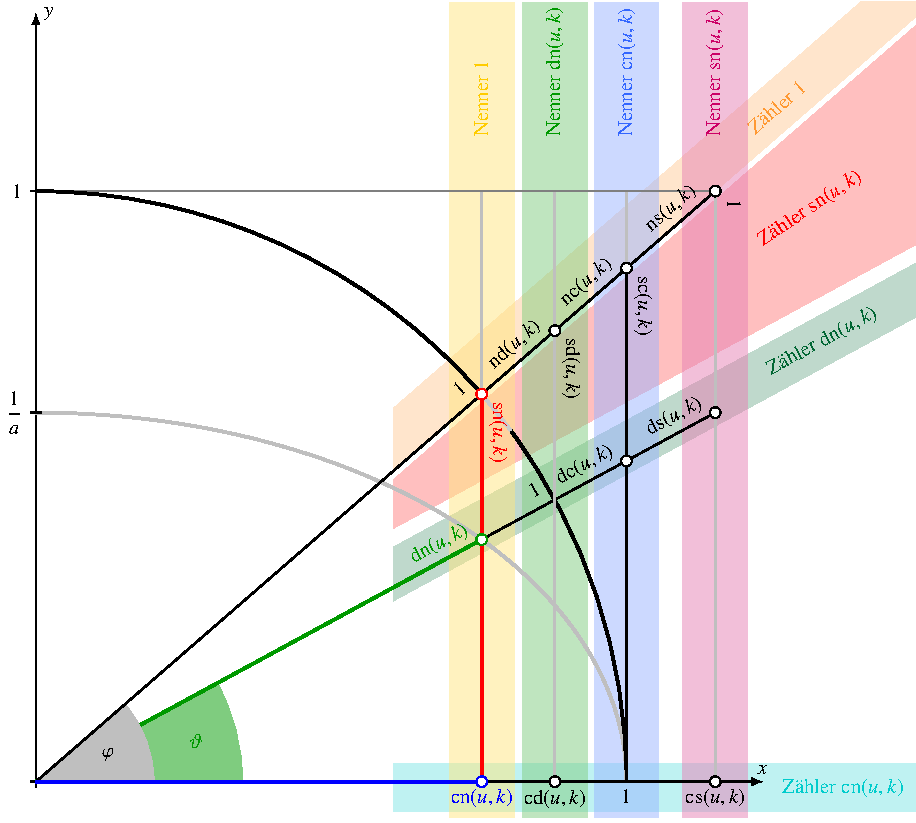
\includegraphics[width=\textwidth]{chapters/110-elliptisch/images/jacobi12.pdf}
\caption{Die Verhältnisse der Funktionen
$\operatorname{sn}(u,k)$,
$\operatorname{cn}(u,k)$
udn
$\operatorname{dn}(u,k)$
geben Anlass zu neun weitere Funktionen, die sich mit Hilfe
des Strahlensatzes geometrisch interpretieren lassen.
\label{buch:elliptisch:fig:jacobi12}}
\end{figure}
\begin{table}
\centering
\renewcommand{\arraystretch}{2.5}
\begin{tabular}{|>{$\displaystyle}c<{$}|>{$\displaystyle}c<{$}>{$\displaystyle}c<{$}>{$\displaystyle}c<{$}>{$\displaystyle}c<{$}|}
\hline
\cdot &
\frac{1}{1} &
\frac{1}{\operatorname{sn}(u,k)} &
\frac{1}{\operatorname{cn}(u,k)} &
\frac{1}{\operatorname{dn}(u,k)} 
\\[5pt]
\hline
1&
&%\operatorname{nn}(u,k)=\frac{1}{1} &
\operatorname{ns}(u,k)=\frac{1}{\operatorname{sn}(u,k)} &
\operatorname{nc}(u,k)=\frac{1}{\operatorname{cn}(u,k)} &
\operatorname{nd}(u,k)=\frac{1}{\operatorname{dn}(u,k)}
\\
\operatorname{sn}(u,k) &
\operatorname{sn}(u,k)=\frac{\operatorname{sn}(u,k)}{1}&
&%\operatorname{ss}(u,k)=\frac{\operatorname{sn}(u,k)}{\operatorname{sn}(u,k)}&
\operatorname{sc}(u,k)=\frac{\operatorname{sn}(u,k)}{\operatorname{cn}(u,k)}&
\operatorname{sd}(u,k)=\frac{\operatorname{sn}(u,k)}{\operatorname{dn}(u,k)}
\\
\operatorname{cn}(u,k) &
\operatorname{cn}(u,k)=\frac{\operatorname{cn}(u,k)}{1} &
\operatorname{cs}(u,k)=\frac{\operatorname{cn}(u,k)}{\operatorname{sn}(u,k)}&
&%\operatorname{cc}(u,k)=\frac{\operatorname{cn}(u,k)}{\operatorname{cn}(u,k)}&
\operatorname{cd}(u,k)=\frac{\operatorname{cn}(u,k)}{\operatorname{dn}(u,k)}
\\
\operatorname{dn}(u,k) &
\operatorname{dn}(u,k)=\frac{\operatorname{dn}(u,k)}{1} &
\operatorname{ds}(u,k)=\frac{\operatorname{dn}(u,k)}{\operatorname{sn}(u,k)}&
\operatorname{dc}(u,k)=\frac{\operatorname{dn}(u,k)}{\operatorname{cn}(u,k)}&
%\operatorname{dd}(u,k)=\frac{\operatorname{dn}(u,k)}{\operatorname{dn}(u,k)}
\\[5pt]
\hline
\end{tabular}
\caption{Zusammenstellung der abgeleiteten Jacobischen elliptischen
Funktionen in hinteren drei Spalten als Quotienten der grundlegenden
Jacobischen elliptischen Funktionen.
Die erste Spalte zum Nenner $1$ enthält die grundlegenden
Jacobischen elliptischen Funktionen.
\label{buch:elliptisch:table:abgeleitetjacobi}}
\end{table}

%
% Die abgeleiteten elliptischen Funktionen
%
\subsubsection{Die abgeleiteten elliptischen Funktionen}
Zusätzlich zu den grundlegenden Jacobischen elliptischen Funktioenn
lassen sich weitere elliptische Funktionen bilden, die unglücklicherweise
die {\em abgeleiteten elliptischen Funktionen} genannt werden.
Ähnlich wie die trigonometrischen Funktionen $\tan\alpha$, $\cot\alpha$,
$\sec\alpha$ und $\csc\alpha$ als Quotienten von $\sin\alpha$ und
$\cos\alpha$ definiert sind, sind die abgeleiteten elliptischen Funktionen
die in Tabelle~\ref{buch:elliptisch:table:abgeleitetjacobi} zusammengestellten
Quotienten der grundlegenden Jacobischen elliptischen Funktionen.
Die Bezeichnungskonvention ist, dass die Funktion $\operatorname{pq}(u,k)$
ein Quotient ist, dessen Zähler durch den Buchstaben p bestimmt ist,
der Nenner durch den Buchstaben q.
Der Buchstabe n steht für eine $1$, die Buchstaben s, c und d stehen für
die Anfangsbuchstaben der grundlegenden Jacobischen elliptischen
Funktionen.
Meint man irgend eine der Jacobischen elliptischen Funktionen, schreibt
man manchmal auch $\operatorname{zn}(u,k)$.

In Abbildung~\ref{buch:elliptisch:fig:jacobi12} sind die Quotienten auch
geometrisch interpretiert.
Der Wert der Funktion $\operatorname{nq}(u,k)$ ist die auf dem Strahl
mit Polarwinkel $\varphi$ abgetragene Länge bis zu den vertikalen
Geraden, die den verschiedenen möglichen Nennern entsprechen.
Entsprechend ist der Wert der Funktion $\operatorname{dq}(u,k)$ die
Länge auf dem Strahl mit Polarwinkel $\vartheta$.

Die Relationen~\ref{buch:elliptisch:eqn:jacobi-relationen}
ermöglichen, jede Funktion $\operatorname{zn}(u,k)$ durch jede
andere auszudrücken.
Die schiere Anzahl solcher Beziehungen macht es unmöglich, sie 
übersichtlich in einer Tabelle zusammenzustellen, daher soll hier
nur an einem Beispiel das Vorgehen gezeigt werden:

\begin{beispiel}
Die Funktion $\operatorname{sc}(u,k)$ soll durch $\operatorname{cd}(u,k)$
ausgedrückt werden.
Zunächst ist 
\[
\operatorname{sc}(u,k)
=
\frac{\operatorname{sn}(u,k)}{\operatorname{cn}(u,k)}
\]
nach Definition.
Im Resultat sollen nur noch $\operatorname{cn}(u,k)$ und
$\operatorname{dn}(u,k)$ vorkommen.
Daher eliminieren wir zunächst die Funktion $\operatorname{sn}(u,k)$
mit Hilfe von \eqref{buch:elliptisch:eqn:jacobi-relationen} und erhalten
\begin{equation}
\operatorname{sc}(u,k)
=
\frac{\sqrt{1-\operatorname{cn}^2(u,k)}}{\operatorname{cn}(u,k)}.
\label{buch:elliptisch:eqn:allgausdruecken}
\end{equation}
Nun genügt es, die Funktion $\operatorname{cn}(u,k)$ durch
$\operatorname{cd}(u,k)$ auszudrücken.
Aus der Definition und der
dritten Relation in \eqref{buch:elliptisch:eqn:jacobi-relationen} 
erhält man
\begin{align*}
\operatorname{cd}^2(u,k)
&=
\frac{\operatorname{cn}^2(u,k)}{\operatorname{dn}^2(u,k)}
=
\frac{\operatorname{cn}^2(u,k)}{k^{\prime2}+k^2\operatorname{cn}^2(u,k)}
\\
\Rightarrow
\qquad
k^{\prime 2}
\operatorname{cd}^2(u,k)
+
k^2\operatorname{cd}^2(u,k)\operatorname{cn}^2(u,k)
&=
\operatorname{cn}^2(u,k)
\\
\operatorname{cn}^2(u,k)
-
k^2\operatorname{cd}^2(u,k)\operatorname{cn}^2(u,k)
&=
k^{\prime 2}
\operatorname{cd}^2(u,k)
\\
\operatorname{cn}^2(u,k)
&=
\frac{
k^{\prime 2}
\operatorname{cd}^2(u,k)
}{
1 - k^2\operatorname{cd}^2(u,k)
}.
\end{align*}
Für den Zähler brauchen wir $1-\operatorname{cn}^2(u,k)$, also
\[
1-\operatorname{cn}^2(u,k)
=
\frac{
1
-
k^2\operatorname{cd}^2(u,k)
-
k^{\prime 2}
\operatorname{cd}^2(u,k)
}{
1
-
k^2\operatorname{cd}^2(u,k)
}
=
\frac{1-\operatorname{cd}^2(u,k)}{1-k^2\operatorname{cd}^2(u,k)}.
\]
Einsetzen in~\eqref{buch:elliptisch:eqn:allgausdruecken} gibt
\begin{align*}
\operatorname{sc}(u,k)
&=
\frac{
\sqrt{1-\operatorname{cd}^2(u,k)}
}{\sqrt{1-k^2\operatorname{cd}^2(u,k)}}
\cdot
\frac{
\sqrt{1 - k^2\operatorname{cd}^2(u,k)}
}{
k'
\operatorname{cd}(u,k)
}
=
\frac{
\sqrt{1-\operatorname{cd}^2(u,k)}
}{
k'
\operatorname{cd}(u,k)
}.
\qedhere
\end{align*}
\end{beispiel}

\subsubsection{Ableitung der abgeleiteten elliptischen Funktionen}
Aus den Ableitungen der grundlegenden Jacobischen elliptischen Funktionen
können mit der Quotientenregel nun auch beliebige Ableitungen der
abgeleiteten Jacobischen elliptischen Funktionen gefunden werden.
Als Beispiel berechnen wir die Ableitung von $\operatorname{sc}(u,k)$.
Sie ist
\begin{align*}
\frac{d}{du}
\operatorname{sc}(u,k)
&=
\frac{d}{du}
\frac{\operatorname{sn}(u,k)}{\operatorname{cn}(u,k)}
=
\frac{
\operatorname{sn}'(u,k)\operatorname{cn}(u,k)
-
\operatorname{sn}(u,k)\operatorname{cn}'(u,k)}{
\operatorname{cn}^2(u,k)
}
\\
&=
\frac{
\operatorname{cn}^2(u,k)\operatorname{dn}(u,k)
+
\operatorname{sn}^2(u,k)\operatorname{dn}(u,k)
}{
\operatorname{cn}^2(u,k)
}
=
\frac{(
\operatorname{sn}^2(u,k)
+
\operatorname{cn}^2(u,k)
)\operatorname{dn}(u,k)}{
\operatorname{cn}^2(u,k)
}
\\
&=
\frac{1}{\operatorname{cn}(u,k)}
\cdot
\frac{\operatorname{dn}(u,k)}{\operatorname{cn}(u,k)}
=
\operatorname{nc}(u,k)
\operatorname{dc}(u,k).
\end{align*}
Man beachte, dass das Quadrat der Nennerfunktion im Resultat
der Quotientenregel zur Folge hat, dass die
beiden Funktionen im Resultat beide den gleichen Nenner haben wie
die Funktion, die abgeleitet wird.

Mit etwas Fleiss kann man nach diesem Muster alle Ableitungen
\begin{equation}
%\small
\begin{aligned}
\operatorname{sn}'(u,k)
&= 
\phantom{-}
\operatorname{cn}(u,k)\,\operatorname{dn}(u,k)
&&\qquad&
\operatorname{ns}'(u,k)
&=
-
\operatorname{cs}(u,k)\,\operatorname{ds}(u,k)
\\
\operatorname{cn}'(u,k)
&= 
-
\operatorname{sn}(u,k)\,\operatorname{dn}(u,k)
&&&
\operatorname{nc}'(u,k)
&=
\phantom{-}
\operatorname{sc}(u,k)\,\operatorname{dc}(u,k)
\\
\operatorname{dn}'(u,k)
&= 
-k^2
\operatorname{sn}(u,k)\,\operatorname{cn}(u,k)
&&&
\operatorname{nd}'(u,k)
&=
\phantom{-}
k^2
\operatorname{sd}(u,k)\,\operatorname{cd}(u,k)
\\
\operatorname{sc}'(u,k)
&=
\phantom{-}
\operatorname{dc}(u,k)\,\operatorname{nc}(u,k)
&&&
\operatorname{cs}'(u,k)
&=
-
\operatorname{ds}(u,k)\,\operatorname{ns}(u,k)
\\
\operatorname{cd}'(u,k)
&=
-k^{\prime2}
\operatorname{sd}(u,k)\,\operatorname{nd}(u,k)
&&&
\operatorname{dc}'(u,k)
&=
\phantom{-}
k^{\prime2}
\operatorname{dc}(u,k)\,\operatorname{nc}(u,k)
\\
\operatorname{ds}'(d,k)
&=
-
\operatorname{cs}(u,k)\,\operatorname{ns}(u,k)
&&&
\operatorname{sd}'(d,k)
&=
\phantom{-}
\operatorname{cd}(u,k)\,\operatorname{nd}(u,k)
\end{aligned}
\label{buch:elliptisch:eqn:alleableitungen}
\end{equation}
finden.
Man beachte, dass in jeder Identität alle Funktionen den gleichen
zweiten Buchstaben haben.

\subsubsection{Weitere Beziehungen}
Für die Jacobischen elliptischen Funktionen lässt sich eine grosse
Zahl weiterer Eigenschaften und Identitäten beweisen.
Zum Beispiel gibt es Aditionstheoreme, die im Grenzfall $k\to 0$ zu
den Additionstheoremen für die trigonometrischen Funktionen werden.
\index{Additionstheorem}%
Ebenso kann man weitere algebraische Identitäten finden.
So lässt sich zum Beispiel die einzige reelle Nullstelle von $x^5+x=w$
mit Jacobischen elliptischen Funktionen darstellen, während es
nicht möglich ist, diese Lösung als Wurzelausdruck zu schreiben.

Die Jacobischen elliptischen Funktionen lassen sich statt auf dem
hier gewählten trigonometrischen Weg auch mit Hilfe der Jacobischen
Theta-Funktionen definieren, die Lösungen einer Wärmeleitungsgleichung
\index{Theta-Funktionen}%
\index{Wärmeleitungs-Gleichung}%
mit geeigneten Randbedingungen sind.
Diese Vorgehensweise hat den Vorteil, ziemlich direkt zu
Reihen- und Produktentwicklungen für die Funktionen zu führen.
Auch die Additionstheorem ergeben sich vergleichsweise leicht.
Dieser Zugang zu den Jacobischen elliptischen Funktionen wird in der
Standardreferenz~\cite{buch:ellfun-applications} gewählt.

Bei anderen speziellen Funktionen waren Reihenentwicklungen ein
wichtiges Hilfsmittel zu deren numerischer Berechnung.
Bei den Jacobischen elliptischen Funktionen ist diese Methode
nicht zielführend.
Im Abschnitt~\ref{buch:elliptisch:subsection:differentialgleichungen}
wird gezeigt, dass Jacobische elliptische Funktionen gewisse nichtlineare
Differentialgleichungen zu lösen ermöglichen.
Dies zeigt auch, dass Jacobischen elliptischen Funktionen
Umkehrfunktionen der elliptischen Integrale sind, die in
Abschnitt~\ref{buch:elliptisch:subsection:agm} mit dem
arithmetisch-geometrischen Mittel berechnet wurden.
Die dort angetroffenen numerischen Schwierigkeiten treten bei der
Berechnung der Umkehrfunktion jedoch nicht auf.

Die grundlegende Mechanik dieser Berechnungsmethode wird auf
Seite~\pageref{buch:elliptisch:jacobi:agm} dargestellt und
und in den Übungsaufgaben
\ref{buch:elliptisch:aufgabe:2} bis \ref{buch:elliptisch:aufgabe:5}
etwas näher untersucht wird.

Aus der Theorie das arithmetisch-geometrischen Mittels lässt sich
die sogenannte Landen-Trans\-formation herleiten.
\index{Landen-Transformation}%
Sie stellt eine Verbindung zwischen
den Werten der elliptischen Funktionen zu verschiedenen Moduli $k$ her.
Sie ist die Basis aller effizienten Berechnungsmethoden.


% algebraische Beziehungen \\
% Additionstheoreme \\
% Perioden
% use https://math.stackexchange.com/questions/3013692/how-to-show-that-jacobi-sine-function-is-doubly-periodic



%
% 22-dglsol.tex -- Lösung von Differentialgleichungen
%
% (c) 2021 Prof Dr Andreas Müller, OST Ostschweizer Fachhochschule
%

%
% Lösung von Differentialgleichungen
%
\subsection{Lösungen von Differentialgleichungen
\label{buch:elliptisch:subsection:differentialgleichungen}}
Die elliptischen Funktionen ermöglichen die Lösung gewisser nichtlinearer
Differentialgleichungen in geschlossener Form.
Ziel dieses Abschnitts ist, Differentialgleichungen der Form
\(
\dot{x}(t)^2
=
P(x(t))
\)
mit einem Polynom $P$ vierten Grades oder
\(
\ddot{x}(t)
=
p(x(t))
\)
mit einem Polynom dritten Grades als rechter Seite lösen zu können.

%
% Die Differentialgleichung der elliptischen Funktionen
%
\subsubsection{Die Differentialgleichungen der elliptischen Funktionen}
Um Differentialgleichungen mit elliptischen Funktion lösen zu
können, muss man als erstes die Differentialgleichungen derselben
finden.
Quadriert man die Ableitungsregel für $\operatorname{sn}(u,k)$, erhält
man
\[
\biggl(\frac{d}{du}\operatorname{sn}(u,k)\biggr)^2
=
\operatorname{cn}(u,k)^2 \operatorname{dn}(u,k)^2.
\]
Die Funktionen auf der rechten Seite können durch $\operatorname{sn}(u,k)$
ausgedrückt werden, dies führt auf die Differentialgleichung
\begin{align*}
\biggl(\frac{d}{du}\operatorname{sn}(u,k)\biggr)^2
&=
\bigl(
1-\operatorname{sn}(u,k)^2
\bigr)
\bigl(
1-k^2 \operatorname{sn}(u,k)^2
\bigr)
\\
&=
k^2\operatorname{sn}(u,k)^4 
-(1+k^2)
\operatorname{sn}(u,k)^2 
+1.
\end{align*}
Für die Funktion $\operatorname{cn}(u,k)$ ergibt die analoge Rechnung
\begin{align*}
\frac{d}{du}\operatorname{cn}(u,k)
&=
-\operatorname{sn}(u,k) \operatorname{dn}(u,k)
\\
\biggl(\frac{d}{du}\operatorname{cn}(u,k)\biggr)^2
&=
\operatorname{sn}(u,k)^2 \operatorname{dn}(u,k)^2
\\
&=
\bigl(1-\operatorname{cn}(u,k)^2\bigr)
\bigl(k^{\prime 2}+k^2 \operatorname{cn}(u,k)^2\bigr)
\\
&=
-k^2\operatorname{cn}(u,k)^4
+
(k^2-k^{\prime 2})\operatorname{cn}(u,k)^2
+
k^{\prime 2}
\intertext{und weiter für $\operatorname{dn}(u,k)$:}
\frac{d}{du}\operatorname{dn}(u,k)
&=
-k^2\operatorname{sn}(u,k)\operatorname{cn}(u,k)
\\
\biggl(
\frac{d}{du}\operatorname{dn}(u,k)
\biggr)^2
&=
\bigl(k^2 \operatorname{sn}(u,k)^2\bigr)
\bigl(k^2 \operatorname{cn}(u,k)^2\bigr)
\\
&=
\bigl(
1-\operatorname{dn}(u,k)^2
\bigr)
\bigl(
\operatorname{dn}(u,k)^2-k^{\prime 2}
\bigr)
\\
&=
-\operatorname{dn}(u,k)^4
+
(1+k^{\prime 2})\operatorname{dn}(u,k)^2
-k^{\prime 2}.
\end{align*}

\begin{table}
\centering
\renewcommand{\arraystretch}{1.7}
\begin{tabular}{|>{$}l<{$}|>{$}l<{$}|>{$}c<{$}|>{$}c<{$}|>{$}c<{$}|}
\hline
\text{Funktion $y=$}&\text{Differentialgleichung}&\alpha&\beta&\gamma\\
\hline
\operatorname{sn}(u,k)
	& y'^2 = \phantom{-}(1-y^2)(1-k^2y^2)
		&k^2&1+k^2&1
\\
\operatorname{cn}(u,k) &y'^2 = \phantom{-}(1-y^2)(k^{\prime2}+k^2y^2)
		&-k^2	&k^2-k^{\prime 2}=2k^2-1&k^{\prime2}
\\
\operatorname{dn}(u,k)
	& y'^2 = -(1-y^2)(k^{\prime 2}-y^2)
		&-1	&1+k^{\prime 2}=2-k^2	&-k^{\prime2}
\\
\hline
\end{tabular}
\caption{Elliptische Funktionen als Lösungsfunktionen für verschiedene
nichtlineare Differentialgleichungen der Art
\eqref{buch:elliptisch:eqn:1storderdglell}.
Die Vorzeichen der Koeffizienten $\alpha$, $\beta$ und $\gamma$
entscheidet darüber, welche Funktion für die Lösung verwendet werden
muss.
\label{buch:elliptisch:tabelle:loesungsfunktionen}}
\end{table}

Die drei grundlegenden Jacobischen elliptischen Funktionen genügen also alle
einer nichtlinearen Differentialgleichung erster Ordnung der selben Art.
Das Quadrat der Ableitung ist ein Polynom vierten Grades der Funktion.
Die Differentialgleichungen sind in der
Tabelle~\ref{buch:elliptisch:tabelle:loesungsfunktionen} zusammengefasst.

%
% Differentialgleichung der abgeleiteten elliptischen Funktionen
%
\subsubsection{Die Differentialgleichung der abgeleiteten elliptischen
Funktionen}
Da auch die Ableitungen der abgeleiteten Jacobischen elliptischen
Funktionen Produkte von genau zwei Funktionen sind, die sich wieder
durch die ursprüngliche Funktion ausdrücken lassen, darf man erwarten,
dass alle elliptischen Funktionen einer ähnlichen Differentialgleichung
genügen.
Um dies besser einzufangen, schreiben wir $\operatorname{pq}(u,k)$,
wenn wir eine beliebige abgeleitete Jacobische elliptische Funktion
meinen.
Für 
$\operatorname{pq}=\operatorname{sn}$,
$\operatorname{pq}=\operatorname{cn}$
und
$\operatorname{pq}=\operatorname{dn}$
wissen wir bereits und erwarten für jede andere Funktion dass
$\operatorname{pq}(u,k)$ auch, dass sie Lösung einer Differentialgleichung
der Form
\begin{equation}
\operatorname{pq}'(u,k)^2
=
\alpha \operatorname{pq}(u,k)^4 + \beta \operatorname{pq}(u,k)^2 + \gamma
\label{buch:elliptisch:eqn:1storderdglell}
\end{equation}
ist,
wobei wir mit $\operatorname{pq}'(u,k)$ die Ableitung von
$\operatorname{pq}(u,k)$ nach dem ersten Argument meinen.
Die Koeffizienten $\alpha$, $\beta$ und $\gamma$ hängen von $k$ ab,
ihre Werte für die grundlegenden Jacobischen elliptischen
sind in Tabelle~\ref{buch:elliptisch:table:differentialgleichungen}
zusammengestellt.

Die Koeffizienten müssen nicht für jede Funktion wieder neu bestimmt
werden, denn für den Kehrwert einer Funktion lässt sich die
Differentialgleichung aus der Differentialgleichung der ursprünglichen
Funktion ermitteln.

%
% Differentialgleichung der Kehrwertfunktion
%
\subsubsection{Differentialgleichung für den Kehrwert einer elliptischen Funktion}
Aus der Differentialgleichung~\eqref{buch:elliptisch:eqn:1storderdglell}
für die Funktion $\operatorname{pq}(u,k)$ kann auch eine
Differentialgleichung für den Kehrwert
$\operatorname{qp}(u,k)=\operatorname{pq}(u,k)^{-1}$
ableiten.
Dazu rechnet man
\[
\operatorname{qp}'(u,k)
=
\frac{d}{du}\frac{1}{\operatorname{pq}(u,k)}
=
\frac{\operatorname{pq}'(u,k)}{\operatorname{pq}(u,k)^2}
\qquad\Rightarrow\qquad
\left\{
\quad
\begin{aligned}
\operatorname{pq}(u,k)
&=
\frac{1}{\operatorname{qp}(u,k)}
\\
\operatorname{pq}'(u,k)
&=
\frac{\operatorname{qp}'(u,k)}{\operatorname{qp}(u,k)^2}
\end{aligned}
\right.
\]
und setzt in die Differentialgleichung ein:
\begin{align*}
\biggl(
\frac{
\operatorname{qp}'(u,k)
}{
\operatorname{qp}(u,k)^2
}
\biggr)^2
&=
\alpha \frac{1}{\operatorname{qp}(u,k)^4}
+
\beta \frac{1}{\operatorname{qp}(u,k)^2}
+
\gamma.
\end{align*}
Nach Multiplikation mit $\operatorname{qp}(u,k)^4$ erhält man den
folgenden Satz.

\begin{satz}
\index{Satz!Differentialgleichung von $1/\operatorname{pq}(u,k)$}%
Wenn die Jacobische elliptische Funktion $\operatorname{pq}(u,k)$
der Differentialgleichung~\eqref{buch:elliptisch:eqn:1storderdglell}
genügt, dann genügt der Kehrwert
$\operatorname{qp}(u,k) = 1/\operatorname{pq}(u,k)$ der Differentialgleichung
\begin{equation}
(\operatorname{qp}'(u,k))^2
= 
\gamma \operatorname{qp}(u,k)^4
+
\beta \operatorname{qp}(u,k)^2
+
\alpha
\label{buch:elliptisch:eqn:kehrwertdgl}
\end{equation}
\end{satz}

\begin{table}
\centering
\def\lfn#1{\multicolumn{1}{|l|}{#1}}
\def\rfn#1{\multicolumn{1}{r|}{#1}}
\renewcommand{\arraystretch}{1.3}
\begin{tabular}{l|>{$}c<{$}>{$}c<{$}>{$}c<{$}|r}
\cline{1-4}
\lfn{Funktion}
         &  \alpha   & \beta     &    \gamma  &\\
\hline
\lfn{sn}&    k^2    & -(1+k^2)  &      1     &\rfn{ns}\\
\lfn{cn}&   -k^2    & -(1-2k^2) &    1-k^2   &\rfn{nc}\\
\lfn{dn}&     1     &  2-k^2    &   -(1-k^2) &\rfn{nd}\\
\hline
\lfn{sc}&   1-k^2   &  2-k^2    &      1     &\rfn{cs}\\
\lfn{sd}&-k^2(1-k^2)&-(1-2k^2)  &       1    &\rfn{ds}\\
\lfn{cd}&    k^2    &-(1+k^2)   &      1     &\rfn{dc}\\
\hline 
                 &   \gamma  & \beta     &   \alpha   &\rfn{Reziproke}\\
\cline{2-5}
\end{tabular}
\caption{Koeffizienten der Differentialgleichungen für die Jacobischen
elliptischen Funktionen.
Der Kehrwert einer Funktion hat jeweils die Differentialgleichung der
ursprünglichen Funktion, in der die Koeffizienten $\alpha$ und $\gamma$
vertauscht worden sind.
\label{buch:elliptisch:table:differentialgleichungen}}
\end{table}

%
% Differentialgleichung zweiter Ordnung
%
\subsubsection{Differentialgleichung zweiter Ordnung}
Leitet man die Differentialgleichung~\eqref{buch:elliptisch:eqn:1storderdglell}
nochmals nach $u$ ab, erhält man die Differentialgleichung
\[
2\operatorname{pq}''(u,k)\operatorname{pq}'(u,k)
=
4\alpha \operatorname{pq}(u,k)^3\operatorname{pq}'(u,k) + 2\beta \operatorname{pq}'(u,k)\operatorname{pq}(u,k).
\]
Teilt man auf beiden Seiten durch $2\operatorname{pq}'(u,k)$,
bleibt die nichtlineare
Differentialgleichung
\[
\frac{d^2\operatorname{pq}}{du^2}
=
\beta \operatorname{pq} + 2\alpha \operatorname{pq}^3.
\]
Dies ist die Gleichung eines harmonischen Oszillators mit einer 
Anharmonizität der Form $2\alpha z^3$.



%
% Jacobischen elliptische Funktionen und elliptische Integrale
%
\subsubsection{Jacobische elliptische Funktionen als elliptische Integrale}
Die in Tabelle~\ref{buch:elliptisch:tabelle:loesungsfunktionen}
zusammengestellten Differentialgleichungen ermöglichen nun, den
Zusammenhang zwischen den Funktionen 
$\operatorname{sn}(u,k)$, $\operatorname{cn}(u,k)$ und $\operatorname{dn}(u,k)$
und den unvollständigen elliptischen Integralen herzustellen.
Die Differentialgleichungen sind alle von der Form
\begin{equation}
\biggl(
\frac{d y}{d u}
\biggr)^2
=
p(u),
\label{buch:elliptisch:eqn:allgdgl}
\end{equation}
wobei $p(u)$ ein Polynom vierten Grades in $y$ ist.
Diese Differentialgleichung lässt sich mit Separation lösen.
Dazu zieht man aus~\eqref{buch:elliptisch:eqn:allgdgl} die
Wurzel
\begin{align}
\frac{dy}{du}
=
\sqrt{p(y)}
\notag
\intertext{und trennt die Variablen. Man erhält}
\int\frac{dy}{\sqrt{p(y)}} = u+C.
\label{buch:elliptisch:eqn:yintegral}
\end{align}
Solange $p(y)>0$ ist, ist der Integrand auf der linken Seite
von~\eqref{buch:elliptisch:eqn:yintegral} ebenfalls positiv und
das Integral ist eine monoton wachsende Funktion $F(y)$.
Insbesondere ist $F(y)$ invertierbar.
Die Lösung $y(u)$ der Differentialgleichung~\eqref{buch:elliptisch:eqn:allgdgl}
ist daher 
\[
y(u) = F^{-1}(u+C).
\]
Die Jacobischen elliptischen Funktionen sind daher inverse Funktionen
der unvollständigen elliptischen Integrale.

\begin{beispiel}
Die Differentialgleichung der Funktion $y=\operatorname{sn}(u,k)$ ist
\[
(y')^2
=
(1-y^2)(1-k^2y^2).
\]
Aus \eqref{buch:elliptisch:eqn:yintegral} folgt daher, dass
\[
u+C
=
\int\frac{dy}{(1-y^2)(1-k^2y^2)}.
\]
Das Integral ist das unvollständige elliptische Integral erster Art.
Mit der Wahl der Konstanten $C$ so, dass $y(0)=0$ ist, ist
$y(u)=\operatorname{sn}(u,k)$ daher die Umkehrfunktion von
$y\mapsto F(y,k)=u$.
\end{beispiel}

%
% Numerische Berechnung mit dem arithmetisch-geometrischen Mittel
%
\subsubsection{Numerische Berechnung mit dem arithmetisch-geometrischen Mittel
\label{buch:elliptisch:jacobi:agm}}
\begin{table}
\centering
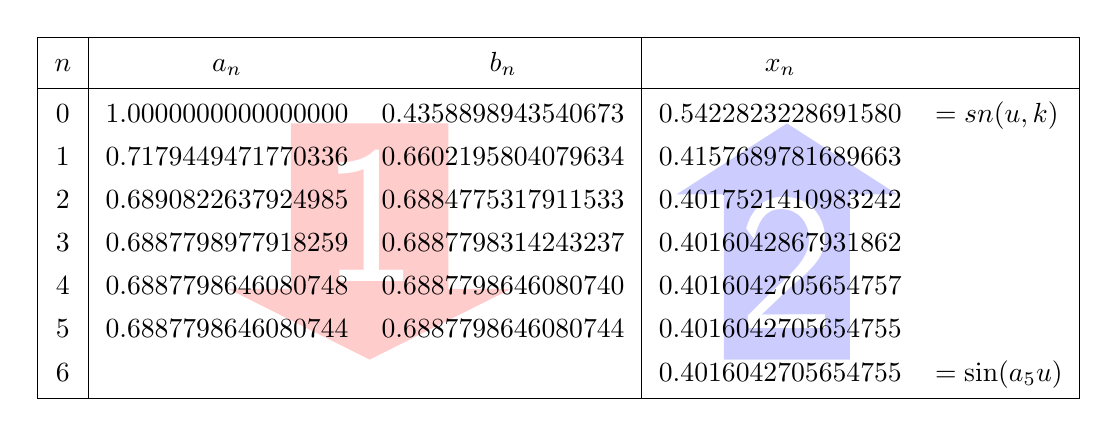
\begin{tikzpicture}[>=latex,thick]

\begin{scope}[xshift=-2.4cm,yshift=1.2cm]
\fill[color=red!20]
	(-1.0,0) -- (-1.0,-2.1) -- (-1.8,-2.1) -- (0,-3.0)
	-- (1.8,-2.1) -- (1.0,-2.1) -- (1.0,0) -- cycle;
\node[color=white] at (0,-1.2) [scale=7] {\sf 1};
\end{scope}

\begin{scope}[xshift=2.9cm,yshift=-1.8cm]
\fill[color=blue!20]
	(0.8,0) -- (0.8,2.1) -- (1.4,2.1) -- (0,3.0) -- (-1.4,2.1)
	-- (-0.8,2.1) -- (-0.8,0) -- cycle;
\node[color=white] at (0,1.2) [scale=7] {\sf 2};
\end{scope}

\node at (0,0) {
\begin{tabular}{|>{$}c<{$}|>{$}c<{$}>{$}c<{$}|>{$}c<{$}>{$}l<{$}|}
\hline
n & a_n                & b_n                  & x_n              &
\mathstrut\text{\vrule height12pt depth6pt width0pt}\\
\hline
0 & 1.0000000000000000 & 0.4358898943540673 & 0.5422823228691580 & = \operatorname{sn}(u,k)%
\mathstrut\text{\vrule height12pt depth0pt width0pt}\\
1 & 0.7179449471770336 & 0.6602195804079634 & 0.4157689781689663 & \mathstrut\\
2 & 0.6890822637924985 & 0.6884775317911533 & 0.4017521410983242 & \mathstrut\\
3 & 0.6887798977918259 & 0.6887798314243237 & 0.4016042867931862 & \mathstrut\\
4 & 0.6887798646080748 & 0.6887798646080740 & 0.4016042705654757 & \mathstrut\\
5 & 0.6887798646080744 & 0.6887798646080744 & 0.4016042705654755 & \mathstrut\\
6 &                    &                    & 0.4016042705654755 & = \sin(a_5u) 
\mathstrut\text{\vrule height0pt depth6pt width0pt}\\
\hline
\end{tabular}
};
\end{tikzpicture}
\caption{Berechnung von $\operatorname{sn}(u,k)$ für $u=0.6$ und $k=0.$2
mit Hilfe des arithmetisch-geo\-me\-tri\-schen Mittels.
In der ersten Phase des Algorithmus (rot) wird die Folge der arithmetischen
\index{Algorithmus!arithmetisch-geometrisches Mittel}%
und geometrischen Mittel berechnet, in der zweiten Phase die
Approximationen von $x_0=\operatorname{sn}(u,k)$.
Bei $n=5$ erreicht die Iteration des arithmetisch-geometrischen Mittels
Maschinengenauigkeit, was sich auch darin äussert, dass sich $x_5$ und
$x_6=\sin(a_5u)$ nicht unterscheiden.
\label{buch:elliptisch:agm:table:snberechnung}}
\end{table}
In Abschnitt~\ref{buch:elliptisch:subsection:agm} auf
Seite~\pageref{buch:elliptisch:subsubection:berechnung-fxk-agm}
wurde erklärt, wie das unvollständige elliptische Integral $F(x,k)$ mit 
Hilfe des arithmetisch-geometrischen Mittels berechnet werden kann.
\index{Algorithmus!arithmetisch-geometrisches Mittel}%
\index{arithmetisch-geometrisches Mittel!Algorithmus}%
Da $\operatorname{sn}^{-1}(x,k) = F(x,k)$ die Umkehrfunktion ist, kann
man den Algorithmus auch zur Berechnung von $\operatorname{sn}(u,k)$ 
verwenden.
Dazu geht man wie folgt vor:
\begin{enumerate}
\item
$k'=\sqrt{1-k^2}$.
\item
Berechne die Folgen des arithmetisch-geometrischen Mittels
$a_n$ und $b_n$ mit $a_0=1$ und $b_0=k'$, bis zum Folgenindex $N$,
bei dem ausreichende Konvergenz eintegreten ist.
\item
Setze $x_N = \sin(a_N \cdot u)$.
\item
Berechnet für absteigende $n=N-1,N-2,\dots$ die Folge $x_n$ mit Hilfe
der Rekursionsformel
\begin{equation}
x_{n}
=
\frac{2a_nx_{n+1}}{a_n+b_n+(a_n-b_n)x_{n+1}^2},
\label{buch:elliptisch:agm:xnrek}
\end{equation}
die aus \eqref{buch:elliptisch:agm:subst}
durch die Substitution $x_n = \sin t_n$ entsteht.
\item
Setze $\operatorname{sn}(u,k) = x_0$.
\end{enumerate}
Da die Formel \eqref{buch:elliptisch:agm:xnrek} nicht unter den
numerischen Stabilitätsproblemen leidet, die früher auf
Seite~\pageref{buch:elliptisch:agm:ellintegral-stabilitaet}
diskutiert wurden, ist die Berechnung stabil und sehr schnell.
Tabelle~\ref{buch:elliptisch:agm:table:snberechnung}
zeigt die Berechnung am Beispiel $u=0.6$ und $k=0.2$.

%
% Pole und Nullstellen der Jacobischen elliptischen Funktionen
%
\subsubsection{Pole und Nullstellen der Jacobischen elliptischen Funktionen}
\begin{figure}
\centering
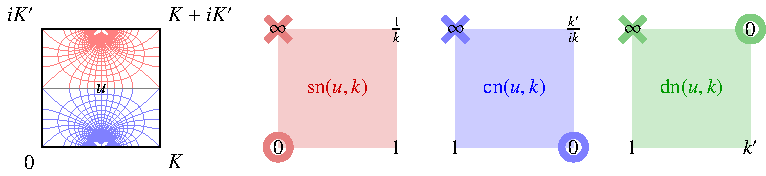
\includegraphics{chapters/110-elliptisch/images/ellpolnul.pdf}
\caption{Werte der grundlegenden Jacobischen elliptischen Funktionen
$\operatorname{sn}(u,k)$,
$\operatorname{cn}(u,k)$
und
$\operatorname{dn}(u,k)$
in den Ecken des Rechtecks mit Ecken $(0,0)$ und $(K,K+iK')$.
Links der Definitionsbereich, rechts die Werte der drei Funktionen.
Pole sind mit einem Kreuz ($\times$) bezeichnet, Nullstellen mit einem
Kreis ($\ocircle$).
\label{buch:elliptisch:fig:ellpolnul}}
\end{figure}
\begin{figure}
\centering
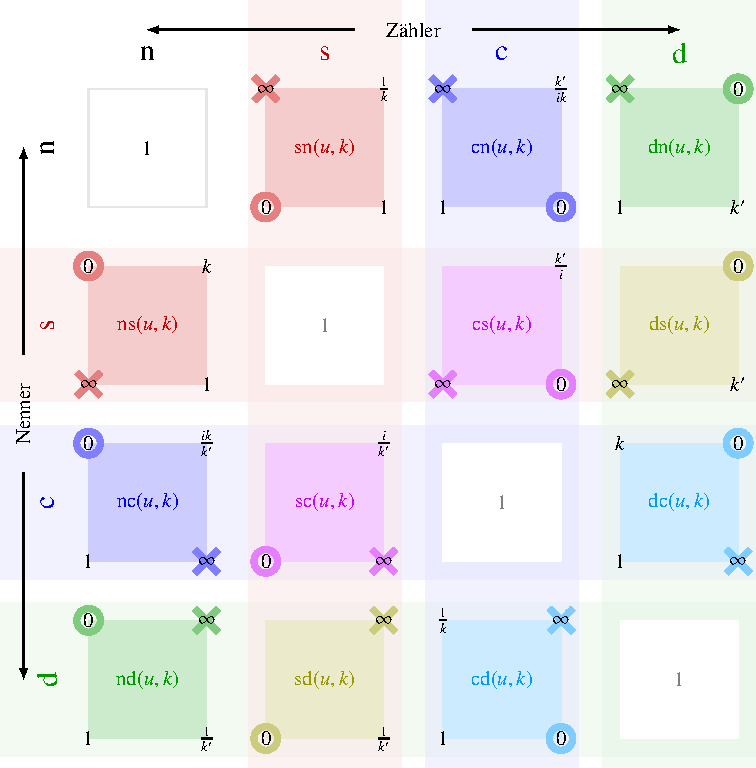
\includegraphics{chapters/110-elliptisch/images/ellall.pdf}
\caption{Pole und Nullstellen aller Jacobischen elliptischen Funktionen
mit den gleichen Darstellungskonventionen wie in
Abbildung~\ref{buch:elliptisch:fig:ellpolnul}
\label{buch:elliptisch:fig:ellall}}
\end{figure}
\begin{figure}
\centering
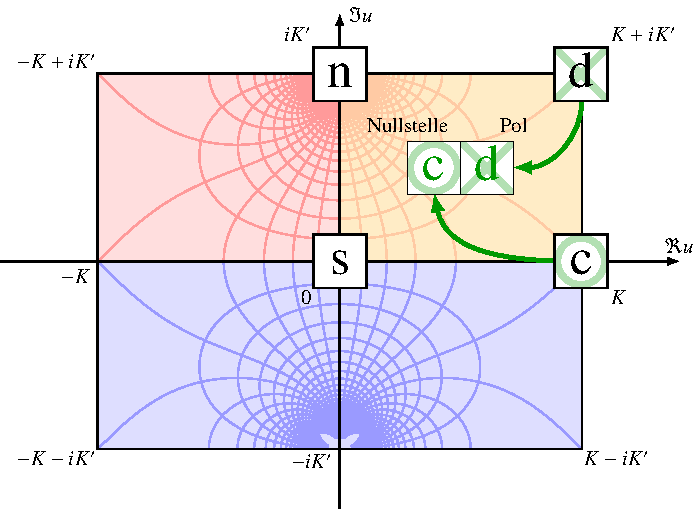
\includegraphics{chapters/110-elliptisch/images/ellselection.pdf}
\caption{Auswahl einer Jacobischen elliptischen Funktion mit bestimmten
Nullstellen und Polen.
Nullstellen und Pole können in jeder der vier Ecken des fundamentalen
Rechtecks (gelb, oberer rechter Viertel des Periodenrechtecks) liegen.
Der erste Buchstabe des Namens der gesuchten Funktion ist der Buchstabe
der Ecke der Nullstelle, der zweite Buchstabe ist der Buchstabe der
Ecke des Poles.
Im Beispiel die Funktion $\operatorname{cd}(u,k)$, welche eine
Nullstelle in $K$ hat und einen Pol in $K+iK'$.
\label{buch:elliptisch:fig:selectell}}
\end{figure}
Für die Funktion $y=\operatorname{sn}(u,k)$ erfüllt die Differentialgleichung
\[
\frac{dy}{du}
=
\sqrt{(1-y^2)(1-k^2y^2)},
\]
welche mit dem unbestimmten Integral
\begin{equation}
u + C = \int\frac{dy}{\sqrt{(1-y^2)(1-k^2y^2)}}
\label{buch:elliptisch:eqn:uyintegral}
\end{equation}
gelöst werden kann.
Der Wertebereich des Integrals in \eqref{buch:elliptisch:eqn:uyintegral}
wurde bereits in
Abschnitt~\ref{buch:elliptisch:subsection:unvollstintegral}
auf Seite~\pageref{buch:elliptische:subsubsection:wertebereich}
diskutiert.
Daraus können jetzt Nullstellen und Pole der Funktion $\operatorname{sn}(u,k)$
und mit Hilfe von Tabelle~\ref{buch:elliptisch:fig:jacobi-relationen}
auch für $\operatorname{cn}(u,k)$ und $\operatorname{dn}(u,k)$
abgelesen werden:
\begin{equation}
\begin{aligned}
\operatorname{sn}(0,k)&=0
&&\qquad&
\operatorname{cn}(0,k)&=1
&&\qquad&
\operatorname{dn}(0,k)&=1
\\
\operatorname{sn}(iK',k)&=\infty
&&\qquad&
\operatorname{cn}(iK',k)&=\infty
&&\qquad&
\operatorname{dn}(iK',k)&=\infty
\\
\operatorname{sn}(K,k)&=1
&&\qquad&
\operatorname{cn}(K,k)&=0
&&\qquad&
\operatorname{dn}(K,k)&=k'
\\
\operatorname{sn}(K+iK',k)&=\frac{1}{k}
&&\qquad&
\operatorname{cn}(K+iK',k)&=\frac{k'}{ik}
&&\qquad&
\operatorname{dn}(K+iK',k)&=0.
\end{aligned}
\label{buch:elliptische:eqn:eckwerte}
\end{equation}
Abbildung~\ref{buch:elliptisch:fig:ellpolnul} zeigt diese Werte
an einer schematischen Darstellung des Definitionsbereiches auf.
Daraus lassen sich jetzt auch die Werte der abgeleiteten Jacobischen
elliptischen Funktionen ablesen, Pole und Nullstellen sind in
Abbildung~\ref{buch:elliptisch:fig:ellall}
zusammengestellt.





%
% Differentialgleichung des anharmonischen Oszillators
%
\subsubsection{Differentialgleichung des anharmonischen Oszillators}
Wir möchten die nichtlineare Differentialgleichung
\index{Differentialgleichung!das anharmonischen Oszillators}%
\begin{equation}
\biggl(
\frac{dx}{dt}
\biggr)^2
=
Ax^4+Bx^2 + C
\label{buch:elliptisch:eqn:anhdgl}
\end{equation}
mit Hilfe elliptischer Funktionen lösen.
Wir nehmen also an, dass die gesuchte Lösung eine Funktion der Form
\begin{equation}
x(t) = a\operatorname{zn}(bt,k)
\label{buch:elliptisch:eqn:loesungsansatz}
\end{equation}
ist.
Die erste Ableitung von $x(t)$ ist
\[
\dot{x}(t) 
=
a\operatorname{zn}'(bt,k).
\]

Indem wir diesen Lösungsansatz in die
Differentialgleichung~\eqref{buch:elliptisch:eqn:anhdgl}
einsetzen, erhalten wir
\begin{equation}
a^2b^2 \operatorname{zn}'(bt,k)^2
=
a^4A\operatorname{zn}(bt,k)^4
+
a^2B\operatorname{zn}(bt,k)^2
+C
\label{buch:elliptisch:eqn:dglx}
\end{equation}
Andererseits wissen wir, dass $\operatorname{zn}(u,k)$ einer
Differentialgleichung der Form~\eqref{buch:elliptisch:eqn:1storderdglell}
erfüllt.
Wenn wir \eqref{buch:elliptisch:eqn:dglx} durch $a^2b^2$ teilen, können wir
die rechte Seite von \eqref{buch:elliptisch:eqn:dglx} mit der rechten
Seite von \eqref{buch:elliptisch:eqn:1storderdglell} vergleichen:
\[
\frac{a^2A}{b^2}\operatorname{zn}(bt,k)^4
+
\frac{B}{b^2}\operatorname{zn}(bt,k)^2
+\frac{C}{a^2b^2}
=
\alpha\operatorname{zn}(bt,k)^4
+
\beta\operatorname{zn}(bt,k)^2
+
\gamma\operatorname{zn}(bt,k).
\]
Daraus ergeben sich die Gleichungen
\begin{align}
\alpha &= \frac{a^2A}{b^2},
&
\beta &= \frac{B}{b^2}
&&\text{und}
&
\gamma &= \frac{C}{a^2b^2}
\label{buch:elliptisch:eqn:koeffvergl}
\intertext{oder aufgelöst nach den Koeffizienten der ursprünglichen
Differentialgleichung}
A&=\frac{\alpha b^2}{a^2}
&
B&=\beta b^2
&&\text{und}&
C &= \gamma a^2b^2
\label{buch:elliptisch:eqn:koeffABC}
\end{align}
für die Koeffizienten der Differentialgleichung der zu verwendenden
Funktion.

Man beachte, dass nach \eqref{buch:elliptisch:eqn:koeffvergl} die 
Koeffizienten $A$, $B$ und $C$ die gleichen Vorzeichen haben wie
$\alpha$, $\beta$ und $\gamma$, da in 
\eqref{buch:elliptisch:eqn:koeffvergl} nur mit Quadraten multipliziert
wird, die immer positiv sind.
Diese Vorzeichen bestimmen, welche der Funktionen gewählt werden muss.

In den Differentialgleichungen für die elliptischen Funktionen gibt
es nur den Parameter $k$, der angepasst werden kann.
Es folgt, dass die Gleichungen
\eqref{buch:elliptisch:eqn:koeffvergl} 
auch $a$ und $b$ bestimmen.
Zum Beispiel folgt aus der letzten Gleichung, dass
\[
b = \pm\sqrt{\frac{B}{\beta}}.
\]
Damit folgt dann aus der zweiten
\[
a=\pm\sqrt{\frac{\beta C}{\gamma B}}.
\]
Die verbleibende Gleichung legt $k$ fest.
Das folgende Beispiel illustriert das Vorgehen am Beispiel einer
Gleichung, die Lösungsfunktion $\operatorname{sn}(u,k)$ verlangt.

\begin{beispiel}
Wir nehmen an, dass die Vorzeichen von $A$, $B$ und $C$ gemäss
Tabelle~\ref{buch:elliptisch:tabelle:loesungsfunktionen} verlangen,
dass die Funktion $\operatorname{sn}(u,k)$ für die Lösung verwendet
werden muss.
Die Tabelle sagt dann auch, dass 
$\alpha=k^2$, $\beta=1$ und $\gamma=1$ gewählt werden müssen.
Aus dem Koeffizientenvergleich~\eqref{buch:elliptisch:eqn:koeffvergl}
folgt der Reihe nach
\begin{align*}
b&=\pm \sqrt{B}
\\
a&=\pm \sqrt{\frac{C}{B}}
\\
k^2
&=
\frac{AC}{B^2}.
\end{align*}
Man beachte, dass man $k^2$ durch Einsetzen von
\eqref{buch:elliptisch:eqn:koeffABC}
auch direkt aus den Koeffizienten $\alpha$, $\beta$ und $\gamma$
erhalten kann, nämlich
\[
\frac{AC}{B^2}
=
\frac{\frac{\alpha b^2}{a^2} \gamma a^2b^2}{\beta^2 b^4}
=
\frac{\alpha\gamma}{\beta^2}.
\qedhere
\]
\end{beispiel}

Da alle Parameter im 
Lösungsansatz~\eqref{buch:elliptisch:eqn:loesungsansatz} bereits
festgelegt sind, stellt sich die Frage, woher man einen weiteren
Parameter nehmen kann, mit dem Anfangsbedingungen erfüllen kann.
Die Differentialgleichung~\eqref{buch:elliptisch:eqn:anhdgl} ist
autonom, die Koeffizienten der rechten Seite der Differentialgleichung
sind nicht von der Zeit abhängig. 
Damit ist eine zeitverschobene Funktion $x(t-t_0)$ ebenfalls eine
Lösung der Differentialgleichung.
Die allgmeine Lösung der 
Differentialgleichung~\eqref{buch:elliptisch:eqn:anhdgl} hat
also die Form
\[
x(t) = a\operatorname{zn}(b(t-t_0)),
\]
wobei die Funktion $\operatorname{zn}(u,k)$ auf Grund der Vorzeichen
von $A$, $B$ und $C$ gewählt werden müssen.

Die Übungsaufgaben~\ref{buch:elliptisch:aufgabe:1} ist als
Lernaufgabe konzipiert, mit der die Lösung der Differentialgleichung
des harmonischen Oszillators beispielhaft durchgearbeitet
werden kann.

%
% 23-mathpendel.tex -- Das mathematische Pendel
%
% (c) 2022 Prof Dr Andreas Müller, OST Ostschweizer Fachhochschule
%

\subsection{Das mathematische Pendel
\label{buch:elliptisch:subsection:mathpendel}}
\begin{figure}
\centering
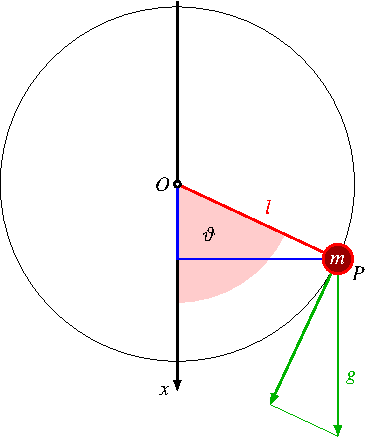
\includegraphics{chapters/110-elliptisch/images/pendel.pdf}
\caption{Mathematisches Pendel
\label{buch:elliptisch:fig:mathpendel}}
\end{figure}
Das in Abbildung~\ref{buch:elliptisch:fig:mathpendel} dargestellte
Mathematische Pendel besteht aus einem Massepunkt der Masse $m$
im Punkt $P$,
der über eine masselose Stange der Länge $l$ mit dem Drehpunkt $O$
verbunden ist.
Das Pendel bewegt sich unter dem Einfluss der Schwerebeschleunigung $g$.

Das Trägheitsmoment des Massepunktes um den Drehpunkt $O$ ist
\(
I=ml^2
\).
Das Drehmoment der Schwerkraft ist
\(M=gl\sin\vartheta\).
Die Bewegungsgleichung wird daher
\[
\begin{aligned}
\frac{d}{dt} I\dot{\vartheta}
&=
M
=
gl\sin\vartheta
\\
ml^2\ddot{\vartheta}
&=
gl\sin\vartheta
&&\Rightarrow&
\ddot{\vartheta}
&=\frac{g}{l}\sin\vartheta.
\end{aligned}
\]
Dies ist eine nichtlineare Differentialgleichung zweiter Ordnung, die
wir nicht unmittelbar mit den Differentialgleichungen erster Ordnung
der elliptischen Funktionen vergleichen können.

Die Differentialgleichungen erster Ordnung der elliptischen Funktionen
enthalten das Quadrat der ersten Ableitung.
In unserem Fall entspricht das einer Gleichung, die $\dot{\vartheta}^2$
enthält.
Der Energieerhaltungssatz kann uns eine solche Gleichung geben.
Die Summe von kinetischer und potentieller Energie muss konstant sein.
Dies führt auf
\begin{equation}
E_{\text{kinetisch}}
+
E_{\text{potentiell}}
=
\frac12I\dot{\vartheta}^2
+
mgl(1-\cos\vartheta)
=
\frac12ml^2\dot{\vartheta}^2
+
mgl(1-\cos\vartheta)
=
E.
\label{buch:elliptisch:mathpendel:energiegleichung}
\end{equation}
Durch Auflösen nach $\dot{\vartheta}$ kann man jetzt die
Differentialgleichung
\[
\dot{\vartheta}^2
=
-
\frac{2g}{l}(1-\cos\vartheta)
+\frac{2E}{ml^2}
\]
finden.
In erster Näherung, d.h. wenn man die rechte Seite bis zu vierten
Potenzen in eine Taylor-Reihe in $\vartheta$ entwickelt,  ist dies
tatsächlich eine Differentialgleichung der Art, wie wir sie für
elliptische Funktionen gefunden haben, wir möchten aber eine exakte
Lösung konstruieren.

Die maximale Energie für eine Bewegung, bei der sich das Pendel gerade
über den höchsten Punkt hinweg zu bewegen vermag, ist 
$E=2lmg$.
Falls $E<2mgl$ ist, erwarten wir Schwingungslösungen, bei denen 
der Winkel $\vartheta$ immer im offenen Interval $(-\pi,\pi)$
bleibt.
Für $E>2mgl$ wird sich das Pendel im Kreis bewegen, für sehr grosse
Energie ist die kinetische Energie dominant, die Verlangsamung im
höchsten Punkt wird immer weniger ausgeprägt sein.


%
% Koordinatentransformation auf elliptische Funktionen
%
\subsubsection{Koordinatentransformation auf elliptische Funktionen}
Wir verwenden als neue Variable 
\begin{align}
y
&=
\sin\frac{\vartheta}2
&&\Rightarrow&
\cos^2\frac{\vartheta}2
&=
1-y^2.
\label{buch:elliptisch:mathpendel:ydef}
\intertext{Die Ableitung ist}
\dot{y}
&=
\frac12\cos\frac{\vartheta}{2}\cdot \dot{\vartheta}
&&\Rightarrow&
\dot{y}^2
&=
\frac14\cos^2\frac{\vartheta}2\cdot\dot{\vartheta}^2.
\label{buch:elliptisch:mathpendel:yabl}
\intertext{%
Man beachte, dass die Koordinate senkrecht zur $x$-Achse in 
Abbildung~\ref{buch:elliptisch:fig:mathpendel} die Auslenkung
$l\sin\vartheta$ ist, $y$ ist also nicht die Auslenkung senkrecht
zur $x$-Achse!
Aus den Halbwinkelformeln finden wir ausserdem
}
\cos\vartheta
&=
1-2\sin^2 \frac{\vartheta}2
=
1-2y^2
&&\Rightarrow&
1-\cos\vartheta
&=
2y^2.
\label{buch:elliptisch:mathpendel:halbwinkel}
\end{align}
Die Grösse $1-\cos\vartheta$ haben wir in der Energiegleichung
\eqref{buch:elliptisch:mathpendel:energiegleichung}
bereits angetroffen.

Die Identitäten 
\eqref{buch:elliptisch:mathpendel:halbwinkel}
%und
%\eqref{buch:elliptisch:mathpendel:ydef}
können wir jetzt in die
Energiegleichung~\eqref{buch:elliptisch:mathpendel:energiegleichung}
einsetzen und erhalten
\begin{align}
\frac12ml^2\dot{\vartheta}^2 + 2mgly^2
&=
E
\intertext{und nach Division durch $2ml^2$}
\frac14 \dot{\vartheta}^2
&=
\frac{E}{2ml^2} - \frac{g}{l}y^2.
\label{buch:elliptisch:mathpendel:thetadgl}
\end{align}
%Der konstante Term auf der rechten Seite ist grösser oder kleiner als
%$1$ je nachdem, ob das Pendel sich im Kreis bewegt oder nicht.
Durch Multiplizieren mit der rechten Gleichung von
\eqref{buch:elliptisch:mathpendel:ydef}
erhalten wir auf der linken Seite einen Ausdruck, den wir
mit Hilfe von \eqref{buch:elliptisch:mathpendel:yabl}
als Funktion von $\dot{y}$ ausdrücken können.
Wir erhalten
\begin{align}
\underbrace{\frac14
\cos^2\frac{\vartheta}2
\cdot
\dot{\vartheta}^2}_{\displaystyle=\dot{y}^2}
&=
(1-y^2)
\biggl(\frac{E}{2ml^2} -\frac{g}{l}y^2\biggr)
\notag
\\
\dot{y}^2
&=
(1-y^2)
\biggl(\frac{E}{2ml^2} -\frac{g}{l}y^2\biggr).
\label{buch:elliptisch:mathpendel:ydgl}
\end{align}
Die letzte Gleichung hat die Form einer Differentialgleichung
für elliptische Funktionen.
Welche Funktion verwendet werden muss, hängt von der relativen
Grösse der Koeffizienten in der zweiten Klammer ab.

%
% Zeittransformation zur Elimination des konstanten Faktors
%
\subsubsection{Zeittransformation}
Die Gleichung~\eqref{buch:elliptisch:mathpendel:ydgl} kann auch in
die Form
\begin{equation}
\frac{2ml^2}{E}\dot{y}^2
=
(1-y^2)\biggl(1-\frac{2mgl}{E}y^2\biggr)
\label{buch:elliptisch:mathpendel:ydgl2}
\end{equation}
gebracht werden.
Der konstante Faktor auf der linken Seite kann wie in der Diskussion
des anharmonischen Oszillators durch eine lineare
Transformation der Zeit zum Verschwinden gebracht werden.
Dazu setzt man $z(t) = y(bt)$ und bekommt
\[
\frac{d}{dt}z(t)
=
\frac{d}{dt}y(bt) \frac{d\,bt}{dt}
=
b\,\dot{y}(bt).
\]
Die Zeit muss also mit dem Faktor $\sqrt{2ml^2/E}$ skaliert werden.

%
% Nullstellen der rechten Seite der Differentialgleichung
%
\subsubsection{Nullstellen der rechten Seite}
Die rechte Seite von \eqref{buch:elliptisch:mathpendel:ydgl2}
hat die beiden Nullstellen $1$ und
\begin{equation}
y_0=\sqrt{\frac{E}{2mgl}}. 
\label{buch:elliptisch:mathpendel:y0}
\end{equation}
Die Differentialgleichung kann damit als
\begin{equation}
\dot{y}^2
=
(1-y^2)\biggl(1-\frac{1}{y_0^2}y^2\biggr)
\label{buch:elliptisch:mathpendel:y0dgl}
\end{equation}
geschrieben werden.
Da die linke Seite $\ge 0$ sein muss, muss 
\(
y\le \min(1,y_0)
\)
sein.
Damit ergeben sich zwei Fälle.
Wenn $y_0<1$ ist, dann schwingt das Pendel.
Der Fall $y_0>1$ entspricht einer Bewegung, bei der das Pendel
um den Punkt $O$ rotiert.
In den folgenden zwei Abschnitten werden die beiden Fälle ausführlicher
diskutiert.


\begin{figure}
\centering
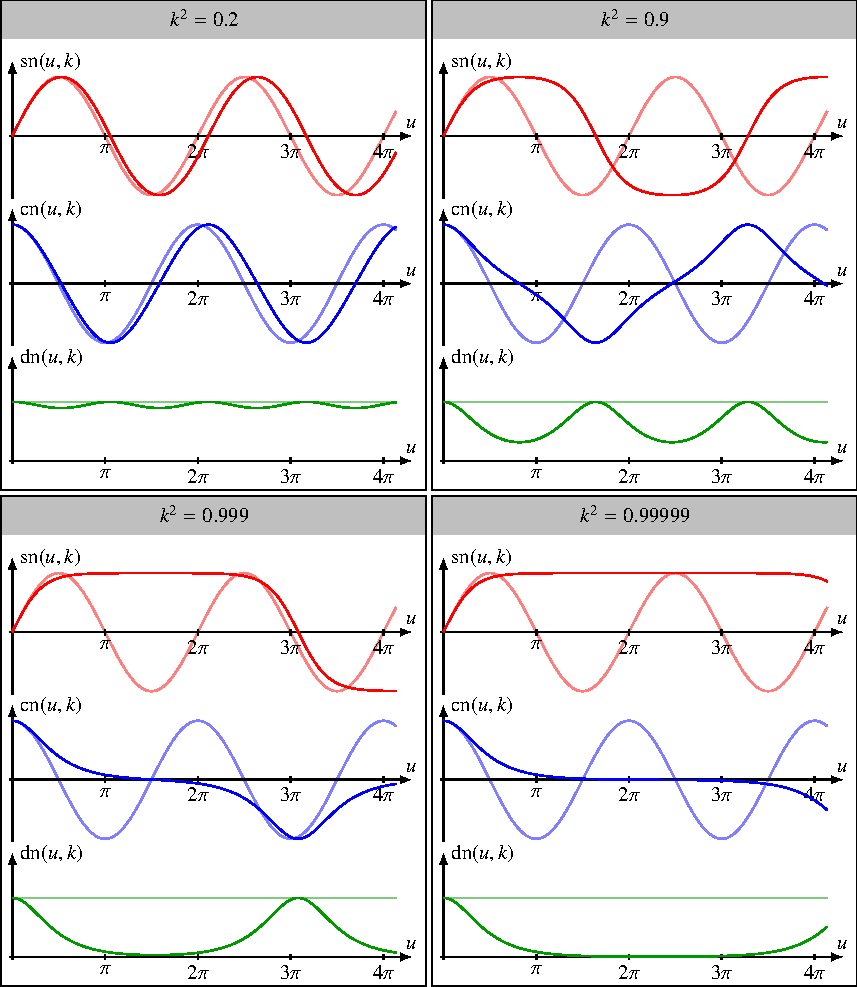
\includegraphics[width=\textwidth]{chapters/110-elliptisch/images/jacobiplots.pdf}
\caption{%
Abhängigkeit der elliptischen Funktionen von $u$ für
verschiedene Werte von $k^2=m$.
Für $m=0$ ist $\operatorname{sn}(u,0)=\sin u$, 
$\operatorname{cn}(u,0)=\cos u$ und $\operatorname{dn}(u,0)=1$, diese
sind in allen Plots in einer helleren Farbe eingezeichnet.
Für kleine Werte von $m$ weichen die elliptischen Funktionen nur wenig
von den trigonometrischen Funktionen ab,
es ist aber klar erkennbar, dass die anharmonischen Terme in der
Differentialgleichung die Periode mit steigender Amplitude verlängern.
Sehr grosse Werte von $m$ nahe bei $1$ entsprechen der Situation, dass
die Energie des Pendels fast ausreicht, dass es den höchsten Punkt
erreichen kann, was es für $m$ macht.
\label{buch:elliptisch:fig:jacobiplots}}
\end{figure}

\subsubsection{Der Fall $E>2mgl$}
In diesem Fall ist die zweite Nullstelle $y_0>1$ oder $1/y_0^2 < 1$.
Die Differentialgleichung~\eqref{buch:elliptisch:mathpendel:y0dgl}
sieht ganz ähnlich aus wie die Differentialgleichung der
Funktion $\operatorname{sn}(u,k)$, tatsächlich wird sie zur
Differentialgleichung von $\operatorname{sn}(u,k)$ wenn man
\[
k^2
=
1/y_0^2
=
\frac{2mgl}{E}
\]
wählt.
In diesem Fall ist also $y=\operatorname{sn}(u,1/y_0)$ eine Lösung
der Differentialgleichung, wobei $u$ eine lineare Funktion der Zeit
ist.

Wenn $y_0 \gg 1$ ist, dann ist $k\approx 0$ und die Bewegung ist
entspricht einer gleichförmigen Kreisbewegung.
Je näher $y_0$ an $1$ liegt, desto näher an $1$ ist auch $k$ und
desto grösser wird die Verlangsamung der Bewgung in der Nähe des
Scheitels, das Pendel verweilt sehr lange.
Dies äussert sich in Abbildung~\ref{buch:elliptisch:fig:jacobiplots}
durch die lange Verweildauer der Funktion nahe der Extrema.

%
% Der Fall E < 2mgl
%
\subsubsection{Der Fall $E<2mgl$}
In diesem Fall ist $y_0<1$ und die
Differentialgleichung~\eqref{buch:elliptisch:mathpendel:y0dgl}
sieht zwar immer noch wie eine Differentialgleichung für
$\operatorname{sn}(u,k)$ aus, aber die Lage der Nullstellen
der rechten Seite ist verkehrt.
Indem wir $y=y_0z$ schreiben, erhalten wir 
\begin{equation}
\dot{y}^2
=
y_0^2 \dot{z}^2
=
(1-y_0^2z^2)(1-z^2).
\end{equation}
Wieder kann durch eine lineare Transformation der Zeit der Faktor $y_0^2$
auf der linken Seite zum Verschwinden gebracht werden, es bleibt
die Differentialgleichung der Funktion $\operatorname{sn}(u,k)$
mit $k=y_0$.
Daraus liest man ab, dass $y_0\operatorname{sn}(u,k)$ die Bewegung
des Pendels im oszillatorischen Fall beschreibt, wobei $u$ wieder
eine lineare Funktion der Zeit ist.

Wenn $y_0\ll 1$ ist, dann ist auch $k$ sehr klein und die lineare
Näherung ist sehr gut, das Pendel verhält sich wie ein harmonischer
Oszillator mit einer Sinus-Schwingung als Lösung.
Für $y_0=k$ nahe an $1$ dagegen erreicht die Schwingung fast den
die maximale Höhe und wird dort sehr langsam.
Dies äussert sich in Abbildung~
Dies äussert sich in Abbildung~\ref{buch:elliptisch:fig:jacobiplots}
wiederum durch die lange Verweildauer der Funktion nahe der Extrema.





%
% lemniskate.tex
%
% (c) 2021 Prof Dr Andreas Müller, OST Ostschweizer Fachhochschule
%
\section{Lemniskatischer Sinus
\label{buch:elliptisch:section:lemniskate}}
\rhead{Lemniskatischer Sinus}
Historisch war der {\em lemniskatische Sinus} die erste ellptische
Funktion, die Gauss bereits als 19-jähriger untersucht, aber nicht 
veröffentlich hat.
In diesem Abschnitt soll die Verbindung zu den Jacobischen
elliptischen Funktionen hergestellt werden.

\subsection{Lemniskate
\label{buch:gemotrie:subsection:lemniskate}}
\begin{figure}
\centering
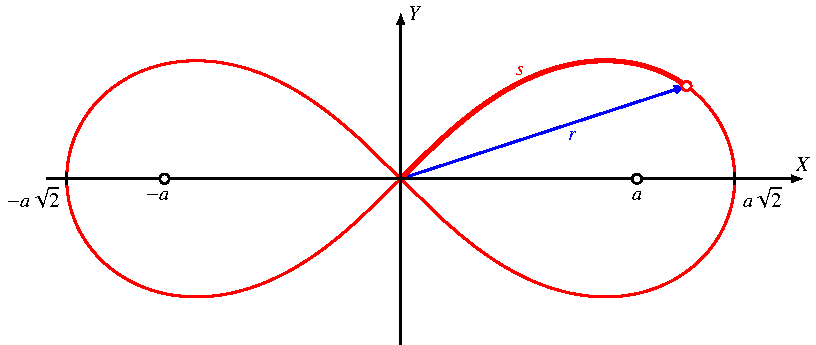
\includegraphics{chapters/110-elliptisch/images/lemniskate.pdf}
\caption{Bogenlänge und Radius der Lemniskate von Bernoulli.
\label{buch:elliptisch:fig:lemniskate}}
\end{figure}
Die Lemniskate von Bernoulli ist die Kurve vierten Grades mit der Gleichung
\begin{equation}
(X^2+Y^2)^2 = 2a^2(X^2-Y^2).
\label{buch:elliptisch:eqn:lemniskate}
\end{equation}
Sie ist in Abbildung~\ref{buch:elliptisch:fig:lemniskate}
dargestellt.
Die beiden Scheitel der Lemniskate befinden sich bei $X_s=\pm a\sqrt{2}$.
Dividiert man die Gleichung der Lemniskate durch $X_s^2=4a^4$ entsteht 
\begin{equation}
\biggl(
\biggl(\frac{X}{a\sqrt{2}}\biggr)^2
+
\biggl(\frac{Y}{a\sqrt{2}}\biggr)^2
\biggr)^2
=
2\frac{a^2}{2a^2}\biggl(
\biggl(\frac{X}{a\sqrt{2}}\biggr)^2
-
\biggl(\frac{Y}{a\sqrt{2}}\biggr)^2
\biggr).
\qquad
\Leftrightarrow
\qquad
(x^2+y^2)^2 = x^2-y^2,
\label{buch:elliptisch:eqn:lemniskatenormiert}
\end{equation}
wobei wir $x=X/a\sqrt{2}$ und $y=Y/a\sqrt{2}$ gesetzt haben.
In dieser Normierung liegen die Scheitel bei $\pm 1$.
Dies ist die Skalierung, die für die Definition des lemniskatischen
Sinus und Kosinus verwendet werden soll.

In Polarkoordinaten $x=r\cos\varphi$ und $y=r\sin\varphi$
gilt nach Einsetzen in \eqref{buch:elliptisch:eqn:lemniskatenormiert}
\begin{equation}
r^4
=
r^2(\cos^2\varphi-\sin^2\varphi)
=
r^2\cos2\varphi
\qquad\Rightarrow\qquad
r^2 = \cos 2\varphi
\label{buch:elliptisch:eqn:lemniskatepolar}
\end{equation}
als Darstellung der Lemniskate in Polardarstellung.
Sie gilt für Winkel $\varphi\in[-\frac{\pi}4,\frac{\pi}4]$ für das
rechte Blatt und $\varphi\in[\frac{3\pi}4,\frac{5\pi}4]$ für das linke
Blatt der Lemniskate.

\subsection{Bogenlänge}
Die Funktionen
\begin{equation}
x(r) = \frac{r}{\sqrt{2}}\sqrt{1+r^2},
\quad
y(r) = \frac{r}{\sqrt{2}}\sqrt{1-r^2}
\label{buch:geometrie:eqn:lemniskateparam}
\end{equation}
erfüllen
\begin{align*}
x(r)^2-y(r)^2
&=
\frac{r^2(1+r^2)}{2}-\frac{r^2(1-r^2)}{2}
\\
&
=
r^4
=
(x(r)^2 + y(r)^2)^2,
\end{align*}
sie stellen also eine Parametrisierung der Lemniskate dar.

Mit Hilfe der Parametrisierung~\eqref{buch:geometrie:eqn:lemniskateparam}
kann man die Länge $s$ des in Abbildung~\ref{buch:elliptisch:fig:lemniskate}
dargestellten Bogens der Lemniskate berechnen.
Dazu benötigt man die Ableitungen nach $r$, die man mit der Produkt- und
Kettenregel berechnen kann:
\begin{align*}
\dot{x}(r)
&=
\frac{\sqrt{1+r^2}}{\sqrt{2}}
+
\frac{r^2}{\sqrt{2}\sqrt{1+r^2}}
&&\Rightarrow&
\dot{x}(r)^2
&=
\frac{1+r^2}{2} +r^2 + \frac{r^4}{2(1+r^2)}
\\
\dot{y}(r)
&=
\frac{\sqrt{1-r^2}}{\sqrt{2}}
-
\frac{r^2}{\sqrt{2}\sqrt{1-r^2}}
&&\Rightarrow&
\dot{y}(r)^2
&=
\frac{1-r^2}{2} -r^2 + \frac{r^4}{2(1-r^2)}
\end{align*}
Die Summe der Quadrate ist
\begin{align*}
\dot{x}(r)^2 + \dot{y}(r)^2
&=
1 + r^4\frac{1-r^2+1+r^2}{2(1+r^2)(1-r^2)}
=
1+r^4\frac{2}{2(1-r^4)}
=
\frac{1-r^4+r^4}{1-r^4}
=
\frac1{1-r^4}.
\end{align*}
Durch Einsetzen in das Integral für die Bogenlänge bekommt man
\begin{equation}
s(r)
=
\int_0^r
\frac{1}{\sqrt{1-t^4}}\,dt.
\label{buch:elliptisch:eqn:lemniskatebogenlaenge}
\end{equation}

%
% Als elliptisches Integral
%
\subsection{Darstellung als elliptisches Integral}
Das unvollständige elliptische Integral erster Art mit Parameter
$k^2=-1$ oder $k=i$ ist
\[
K(r,i)
=
\int_0^x \frac{dt}{\sqrt{(1-t^2)(1-i^2 t^2)}}
=
\int_0^x \frac{dt}{\sqrt{(1-t^2)(1-(-1)t^2)}}
=
\int_0^x \frac{dt}{\sqrt{1-t^4}}
=
s(r).
\]
Der lemniskatische Sinus ist also eine Umkehrfunktion des
elliptischen Integrals erster Art für den speziellen Wert $i$ des
Parameters $k$.

Die Länge des rechten Blattes der Lemniskate wird mit $\varpi$ bezeichnet
und hat den numerischen Wert
\[
\varpi
=
2\int_0^1\sqrt{\frac{1}{1-t^4}}\,dt
=
2.6220575542.
\]
$\varpi$ ist auch als die {\em lemniskatische Konstante} bekannt.
\index{lemniskatische Konstante}%
Der Lemniskatenbogen zwischen dem Nullpunkt und $(1,0)$ hat die Länge
$\varpi/2$.

%
%  Bogenlängenparametrisierung
%
\subsection{Bogenlängenparametrisierung}
Die Lemniskate mit der Gleichung
\[
(X^2+X^2)^2=2(X^2-X^2)
\]
(der Fall $a=1$ in \eqref{buch:elliptisch:eqn:lemniskate})
kann mit Jacobischen elliptischen Funktionen
parametrisiert werden.
Dazu schreibt man
\[
\left.
\begin{aligned}
X(t)
&=
\sqrt{2}\operatorname{cn}(t,k) \operatorname{dn}(t,k)
\\
Y(t)
&=
\phantom{\sqrt{2}}
\operatorname{cn}(t,k) \operatorname{sn}(t,k)
\end{aligned}
\quad\right\}
\qquad\text{mit $k=\displaystyle\frac{1}{\sqrt{2}}$}
\]
und berechnet die beiden Seiten der definierenden Gleichung der
Lemniskate.
Zunächst ist
\begin{align*}
X(t)^2
&=
2\operatorname{cn}(t,k)^2
\operatorname{dn}(t,k)^2
\\
Y(t)^2
&=
\operatorname{cn}(t,k)^2
\operatorname{sn}(t,k)^2
\\
X(t)^2+Y(t)^2
&=
2\operatorname{cn}(t,k)^2
\bigl(
\underbrace{
\operatorname{dn}(t,k)^2
+{\textstyle\frac12}
\operatorname{sn}(t,k)^2
}_{\displaystyle =1}
\bigr)
%\\
%&
=
2\operatorname{cn}(t,k)^2
\\
X(t)^2-Y(t)^2
&=
\operatorname{cn}(t,k)^2
\bigl(
2\operatorname{dn}(t,k)^2 - \operatorname{sn}(t,k)^2
\bigr)
\\
&=
\operatorname{cn}(t,k)^2
\bigl(
2\bigl({\textstyle\frac12}+{\textstyle\frac12}\operatorname{cn}(t,k)^2\bigr)
-
\bigl(1-\operatorname{cn}(t,k)^2\bigr)
\bigr)
\\
&=
2\operatorname{cn}(t,k)^4
\\
\Rightarrow\qquad
(X(t)^2+Y(t)^2)^2
&=
4\operatorname{cn}(t,k)^4
=
2(X(t)^2-Y(t)^2).
\end{align*}
Wir zeigen jetzt, dass dies tatsächlich eine Bogenlängenparametrisierung
der Lemniskate ist.
Dazu berechnen wir die Ableitungen
\begin{align*}
\dot{X}(t)
&=
\sqrt{2}\operatorname{cn}'(t,k)\operatorname{dn}(t,k)
+
\sqrt{2}\operatorname{cn}(t,k)\operatorname{dn}'(t,k)
\\
&=
-\sqrt{2}\operatorname{sn}(t,k)\operatorname{dn}(t,k)^2
-\frac12\sqrt{2}\operatorname{sn}(t,k)\operatorname{cn}(t,k)^2
\\
&=
-\sqrt{2}\operatorname{sn}(t,k)\bigl(
1-{\textstyle\frac12}\operatorname{sn}(t,k)^2
+{\textstyle\frac12}-{\textstyle\frac12}\operatorname{sn}(u,t)^2
\bigr)
\\
&=
\sqrt{2}\operatorname{sn}(t,k)
\bigl(
{\textstyle \frac32}-\operatorname{sn}(t,k)^2
\bigr)
\\
\dot{X}(t)^2
&=
2\operatorname{sn}(t,k)^2
\bigl(
{\textstyle \frac32}-\operatorname{sn}(t,k)^2
\bigr)^2
\\
&=
{\textstyle\frac{9}{2}}\operatorname{sn}(t,k)^2
-
6\operatorname{sn}(t,k)^4
+2\operatorname{sn}(t,k)^6
\\
\dot{Y}(t)
&=
\operatorname{cn}'(t,k)\operatorname{sn}(t,k)
+
\operatorname{cn}(t,k)\operatorname{sn}'(t,k)
\\
&=
-\operatorname{sn}(t,k)^2
\operatorname{dn}(t,k)
+\operatorname{cn}(t,k)^2
\operatorname{dn}(t,k)
\\
&=
\operatorname{dn}(t,k)\bigl(1-2\operatorname{sn}(t,k)^2\bigr)
\\
\dot{Y}(t)^2
&=
\bigl(1-{\textstyle\frac12}\operatorname{sn}(t,k)^2\bigr)
\bigl(1-2\operatorname|{sn}(t,k)^2\bigr)^2
\\
&=
1-{\textstyle\frac{9}{2}}\operatorname{sn}(t,k)^2
+6\operatorname{sn}(t,k)^4
-2\operatorname{sn}(t,k)^6
\\
\dot{X}(t)^2 + \dot{Y}(t)^2
&=
1.
\end{align*}
Dies bedeutet, dass die Bogenlänge zwischen den Parameterwerten $0$ und $s$
\[
\int_0^s
\sqrt{\dot{X}(t)^2 + \dot{Y}(t)^2}
\,dt
=
\int_0^s\,dt
=
s,
\]
der Parameter $t$ ist also ein Bogenlängenparameter.

Die mit dem Faktor $1/\sqrt{2}$ skalierte Standard-Lemniskate mit der
Gleichung
\[
(x^2+y^2)^2 = x^2-y^2
\]
hat daher eine Bogenlängenparametrisierung mit
\begin{equation}
\begin{aligned}
x(t)
&=
\phantom{\frac{1}{\sqrt{2}}}
\operatorname{cn}(\sqrt{2}t,k)\operatorname{dn}(\sqrt{2}t,k)
\\
y(t)
&=
\frac{1}{\sqrt{2}}\operatorname{cn}(\sqrt{2}t,k)\operatorname{sn}(\sqrt{2}t,k)
\end{aligned}
\label{buch:elliptisch:lemniskate:bogenlaenge}
\end{equation}

\subsection{Der lemniskatische Sinus und Kosinus}
Der Sinus Berechnet die Gegenkathete zu einer gegebenen Bogenlänge des
Kreises, er ist die Umkehrfunktion der Funktion, die der Gegenkathete
die Bogenlänge zuordnet.

Daher ist es naheliegend, die Umkehrfunktion von $s(r)$ in 
\eqref{buch:elliptisch:eqn:lemniskatebogenlaenge}
den {\em lemniskatischen Sinus} zu nennen mit der Bezeichnung
$r=\operatorname{sl} s$.

Der Kosinus ist der Sinus des komplementären Winkels.
Auch für die lemniskatische Bogenlänge $s(r)$ lässt sich eine
komplementäre Bogenlänge definieren, nämlich die Bogenlänge zwischen
dem Punkt $(x(r), y(r))$ und $(1,0)$.

Da die Parametrisierung~\eqref{buch:elliptisch:lemniskate:bogenlaenge}
eine Bogenlängenparametrisierung ist, darf man $t=s$ schreiben.
Dann kann man aber auch $r(s)$ daraus berechnen,
es ist
\[
r(s)^2
=
x(s)^2 + y(s)^2
=
\operatorname{cn}(s\sqrt{2},k)^2
\qquad\Rightarrow\qquad
r(s)
=
\operatorname{cn}(s\sqrt{2},k)
\]

\begin{figure}
\centering
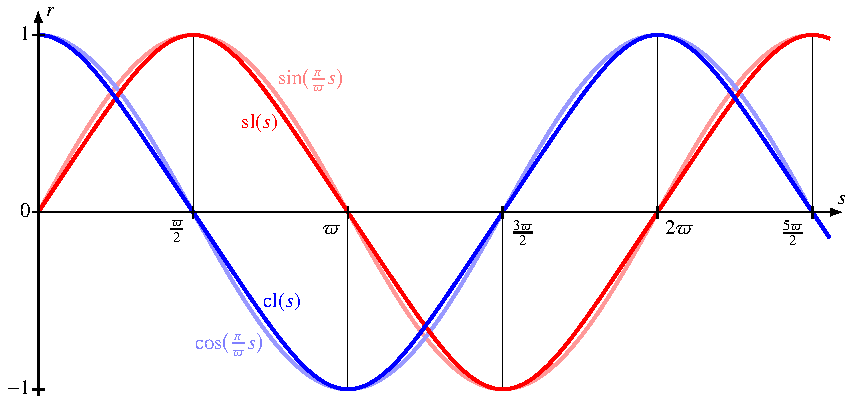
\includegraphics{chapters/110-elliptisch/images/slcl.pdf}
\caption{
Lemniskatischer Sinus und Kosinus sowie Sinus und Kosinus
mit derart skaliertem Argument, dass die Funktionen die gleichen Nullstellen
haben.
\label{buch:elliptisch:figure:slcl}}
\end{figure}


\section*{Übungsaufgaben}
\rhead{Übungsaufgaben}
\aufgabetoplevel{chapters/110-elliptisch/uebungsaufgaben}
\begin{uebungsaufgaben}
%\uebungsaufgabe{0}
\uebungsaufgabe{1}
\uebungsaufgabe{2}
\uebungsaufgabe{3}
\uebungsaufgabe{4}
\uebungsaufgabe{5}
\end{uebungsaufgaben}

